\documentclass[11pt]{article}
\usepackage[margin=1in]{geometry}
\usepackage[utf8]{inputenc}
\usepackage[T1]{fontenc}
\usepackage{lmodern}
\usepackage{graphicx}
\usepackage{float}
\usepackage{booktabs}
\usepackage{amsmath,amssymb}
\usepackage{microtype}
\usepackage{xcolor}
\usepackage{natbib}
\usepackage{hyperref}
\usepackage{url}

\newcommand{\todo}[1]{\textcolor{red}{\textbf{[TODO: #1]}}}
\title{How Chain-of-Thought Rewires Counting:\\From Parallel Aggregation to Serial Retrieval}
\author{
Liang Twist Shan\textsuperscript{1}\quad
Tianyu Hu\textsuperscript{2}\quad
Hao Yan\textsuperscript{3}\quad
Yiqiao Zhong\textsuperscript{3}\\[0.6em]
{\small \textsuperscript{1}School of Mathematical Sciences, Peking University}\\
{\small \textsuperscript{2}Department of Computer Sciences, University of Wisconsin--Madison}\\
{\small \textsuperscript{3}Department of Statistics, University of Wisconsin--Madison}
}
\date{July 21, 2026}

\newcommand{\nt}{\textsc{Direct}}
\newcommand{\traceroute}{\textsc{Trace}}
\newcommand{\ans}{\texttt{<Ans>}}
\newcommand{\think}{\texttt{<Think>}}
\newcommand{\close}{\texttt{</Think>}}

\begin{document}
\maketitle

\begin{abstract}
Why does chain-of-thought (CoT) make counting in long contexts dramatically easier? We show that the answer lies not in a single better count representation, but in a change of computational route. We train matched 3.18M-parameter RoPE transformers from identical initialization and data, varying only whether they answer directly or first emit an indexed trace. Direct answering learns a late, broad-attention mechanism that aggregates many occurrences at the answer site. The trace model instead learns an externalized serial loop: index-conditioned heads retrieve the $k$th occurrence, trace states control successor and stop decisions, and a separate readout converts the completed trace into a count. Query-local ablations, activation patching, residual transplantation, and steering establish the predicted causal links along both routes. Moving the query next to the output raises autoregressive accuracy from 84\% to 96\% and shifts the earliest decodable count state toward an earlier query bottleneck. In 4K-token experiments, Qwen3-8B and Olmo-Hybrid-7B retrieve nearly all relevant records yet often fail to count them directly, while enumeration scaffolds substantially restore accuracy. These results suggest that CoT improves counting by creating an addressable serial interface that separates retrieval, progress, and readout---not merely by adding tokens or exposing a more linearly decodable number state.
\end{abstract}

\section{Introduction}

Chain-of-thought (CoT) and scratchpad prompting can transform the performance of language models on multi-step tasks \citep{nye2021scratchpads,wei2022cot}. Yet the mechanism behind this gain remains underspecified. Extra tokens may simply provide more sequential compute \citep{pfau2024dot}; alternatively, their semantic and positional structure may create a new interface through which a model can route information. Counting relevant items in a long context is a minimal setting in which these accounts make different predictions. A model must retrieve each relevant item, aggregate across items, and map the result to an output token. These operations can succeed or fail independently.

We combine controlled training with realistic needle-in-a-haystack (NIAH) evaluation. The controlled setting trains two transformers from identical initialization on identical prompts and optimizer updates. The only systematic difference is the output representation: one model emits the count directly, while the other emits an ordered index--marker trace before the same count. The realistic setting evaluates 7--8B parameter open models on 4K-token documents with multiple city--score records. This two-scale design lets us use small models for dense causal intervention and large models for external validity.

Our central claim is that the output interface selects between two routes (Figure~\ref{fig:routes}). The \nt{} route uses broad attention at the answer query and writes a count state late in the residual stream. The \traceroute{} route externalizes a loop: a progress state selects the next prompt occurrence, the retrieved marker is written to the trace, and a successor/stop state updates progress. A separate readout then converts trace structure into a scalar answer. We use ``route'' rather than ``circuit'' because some components are localized only to role-level head sets or residual subspaces.

Our contributions are:
\begin{itemize}
    \item We formulate direct aggregation and externalized serial retrieval as intervention-ready hypotheses, distinguishing attention routing from residual content and descriptive decodability from causal control.
    \item In matched synthetic transformers, we close several causal links with query-local ablation, head-output and MLP-feature patching, residual transplantation, and geometry steering. The two output formats yield different learning times, layer locations, and executable count states.
    \item We show that query placement is not a cosmetic prompt change: moving the query after the data rewires nonthinking counting toward an early query bottleneck and improves paired autoregressive accuracy by 12 percentage points.
    \item In realistic 4K NIAH, we separate retrieval from aggregation. Models can retrieve essentially every item while failing to count beyond three; enumeration restores counting, and mechanistic tests in Qwen3-8B support a parallel, dilution-limited direct readout.
\end{itemize}

\begin{figure}[t]
    \centering
    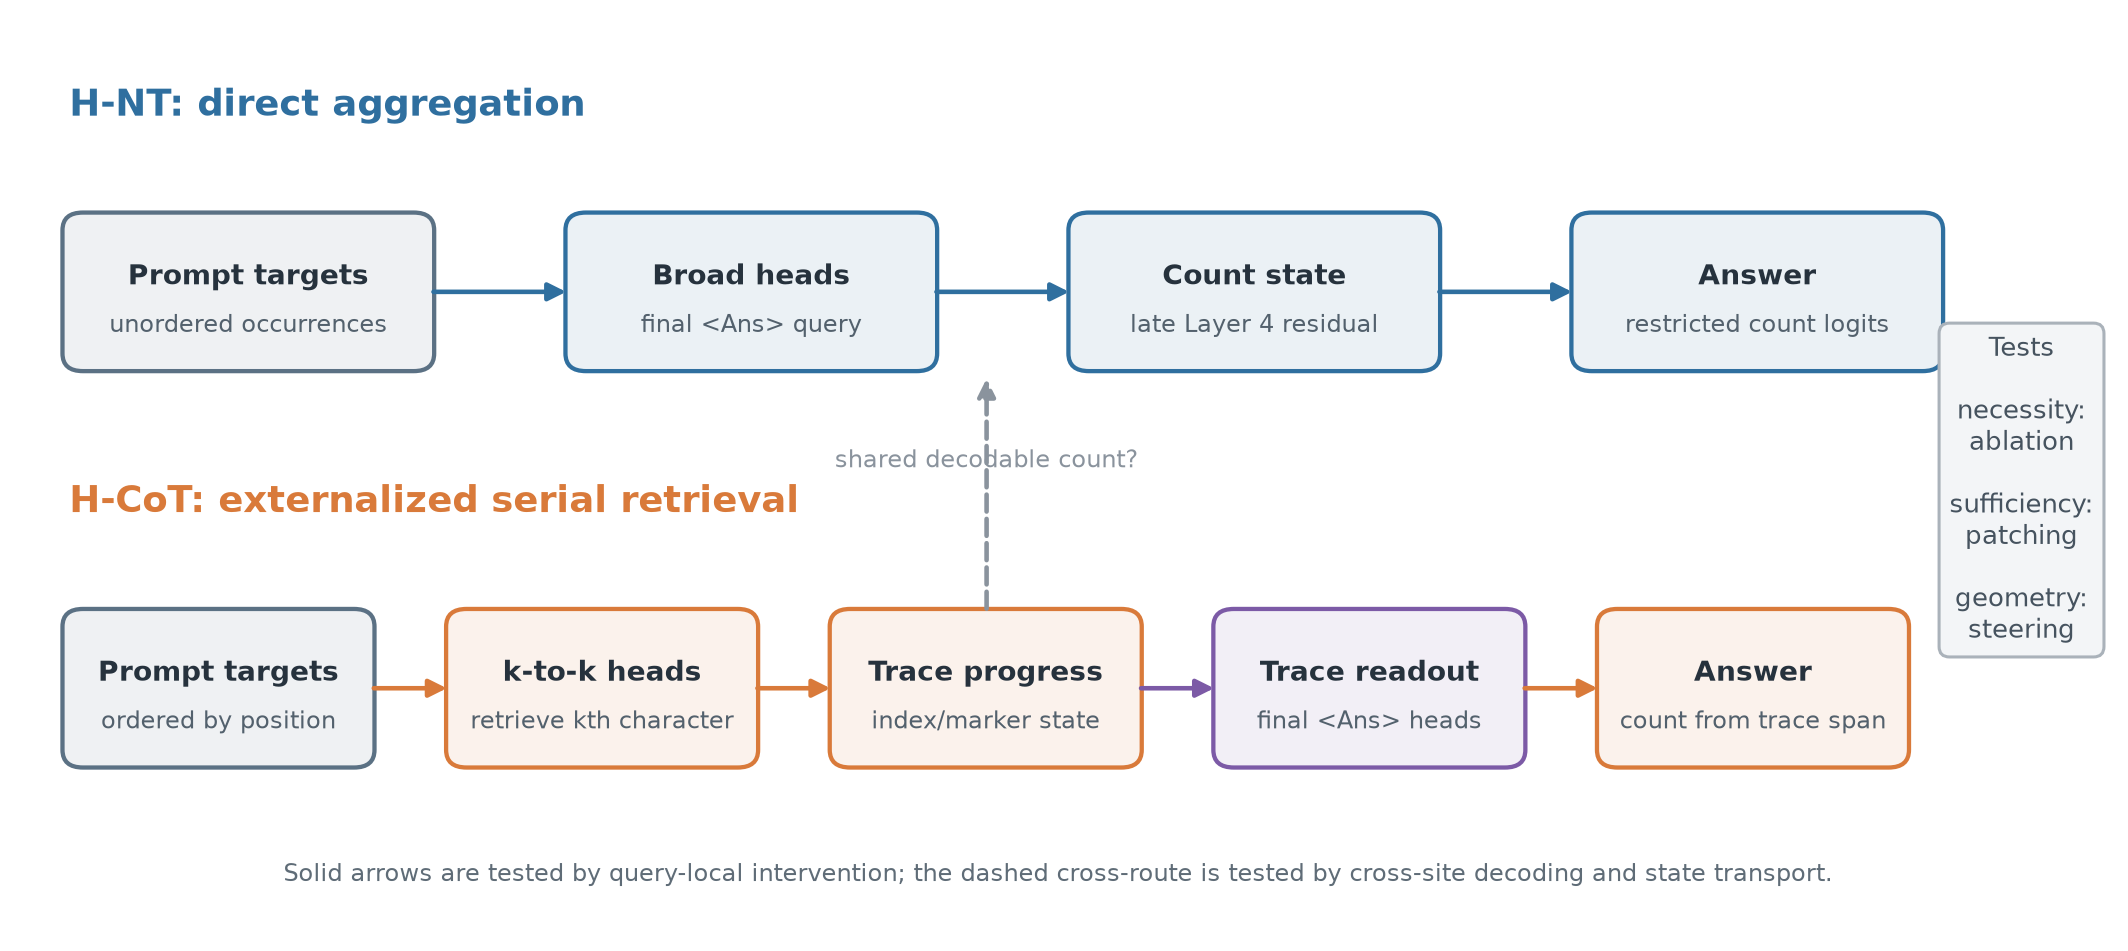
\includegraphics[width=\linewidth]{figures/mechanism_routes.png}
    \caption{Two candidate routes to the same count token. \textbf{Top:} direct answering broadly routes unordered prompt occurrences into a late count state. \textbf{Bottom:} an indexed trace creates a serial $k$-to-$k$ retrieval interface, an explicit progress state, and a separate trace-to-answer readout. Solid arrows are tested by query-local intervention; the dashed cross-route relation is tested only by decoding and state transport.}
    \label{fig:routes}
\end{figure}

\section{Experimental framework}
\label{sec:framework}

\subsection{Task and mechanistic hypotheses}

Let a context contain ordered target occurrences at positions $P=\{p_1,\ldots,p_n\}$. The direct output is the count token $C_n$. The trace output is an ordered sequence $(1,M_1),\ldots,(n,M_n)$ followed by $C_n$, where $M_k$ identifies the target character at $p_k$.

\paragraph{H-NT: direct aggregation.}
At the final \ans{} query, a set of heads distributes attention across multiple $p_k$ and writes aggregate evidence into the residual stream. Later computation converts this evidence into a count-selective state and then into logits over $C_1,\ldots,C_N$. This hypothesis predicts broad target coverage rather than a $k$-specific diagonal, and it predicts late causal count transport at the answer site.

\paragraph{H-CoT: externalized serial retrieval.}
At trace index $k$, a targeted head set retrieves $p_k$ and writes $M_k$. The marker state then supports either successor $k+1$ or \close{}, producing a recurrent dependency
\begin{equation}
    \text{progress } k \rightarrow \text{retrieve } p_k \rightarrow M_k
    \rightarrow (k+1\text{ or stop}) \rightarrow \text{updated progress}.
\end{equation}
A distinct answer-site readout converts the completed trace into $C_n$. The hypothesis predicts $k$-to-$k$ attention, causal control of successor/stop, and separable progress and scalar-count states.

We evaluate each arrow at three levels. \emph{Necessity} asks whether query-local ablation damages the predicted downstream variable. \emph{Local sufficiency} asks whether a clean donor activation restores or transports the variable in a matched corrupt receiver. \emph{Executability} asks whether a residual direction or natural state transplant controls the model's output. Attention maps and linear probes are treated as screening tools, not as standalone causal evidence \citep{zhang2024patching}.

\subsection{Controlled synthetic models}

Each example contains a 256-character Shakespeare window and a three-character target set. The label is the union count of target occurrences, balanced over $n\in\{1,\ldots,10\}$ at evaluation. The query-first layout is
\begin{align*}
    \text{query} \rightarrow \text{data} \rightarrow \text{output},
\end{align*}
with the query in positions 1--5, data in 6--261, and output beginning at 262. The nonthinking output is \ans{} $C_n$; the thinking output begins with \think{}, emits ordered index--marker pairs, closes with \close{}, and then emits \ans{} $C_n$.

Both variants are 4-layer, 4-head causal transformers with $d_{\mathrm{model}}=256$, MLP width 1024, context 384, RoPE base 10,000, no dropout, and 3,180,800 parameters. They share seed 1234, initial weights, training examples and order, AdamW updates, and a 10,000-step budget (batch 128, learning rate $3\times10^{-4}$). The first 1,500 steps optimize the full sequence; subsequent steps optimize task-output tokens only. We save 21 checkpoints at intervals of 500 steps. Final teacher-forced (TF) evaluation uses 50 examples per count and autoregressive (AR) evaluation uses 10 per count. Mechanism head selection and reporting use disjoint prompts.

\todo{Add synthetic-training hardware, wall-clock time, software versions, and the public code/data URL.}

\subsection{Query-position intervention}

The query-last run changes only the interface:
\begin{align*}
    \text{data}_{1:256} \rightarrow \text{query}_{257:261} \rightarrow \text{output}_{262:}.
\end{align*}
Thus output positions, initialization, examples, optimization, and output tokens are fixed. What changes jointly is causal visibility, query-to-output RoPE distance, and a five-position shift of the data. This design measures the total layout effect; it does not by itself identify which of the three subfactors is causal.

\subsection{Realistic 4K NIAH}

We insert $N$ city--score records into Paul Graham essay text, keeping realized context length at 3.82--3.97K tokens. We evaluate Qwen3-8B with thinking disabled \citep{yang2025qwen3} and Olmo-Hybrid-7B \citep{merrill2026olmohybrid} under greedy decoding. Main grids use 30 independent seeds per cell and cover $N=1$--45, seven placement patterns, and three query placements. Three paired output variants isolate operations: \emph{count} emits one integer; \emph{list} emits every city--score pair and measures item recall; \emph{list+count} enumerates before emitting a total. A numbered-enumeration condition makes the external counter explicit. The setup extends NIAH from single-item retrieval to aggregation, in the spirit of RULER \citep{hsieh2024ruler}.

\todo{Add exact model/tokenizer revisions, inference-library versions, licenses, hardware, decoding parameters, and the public prompt archive URL.}

\section{Controlled training reveals two routes}
\label{sec:synthetic}

\subsection{Learning time and representation separate before final behavior}

The thinking model constructs an answer readout before it learns reliable ordered retrieval (Figure~\ref{fig:learning}). By steps 500--1,500, a Layer-2 head already places roughly 84--90\% of final-answer attention on trace tokens, while correct-$k$ prompt retrieval becomes reliable only around steps 4,500--5,000. In contrast, the direct model's broad target coverage and AR accuracy rise together late, with persistent half-rise near step 7,000.

Residual geometry follows the same ordering. At the final checkpoint, thinking count is nearly perfectly linearly decodable at Layer 2 ($R^2=0.998$; nearest-centroid accuracy 1.00). Direct count becomes strongest at Layer 4 ($R^2=0.957$; nearest-centroid accuracy 0.733). Neither geometry is a single global ``$+1$'' number line: mean-first PCA curves, effective dimension changes across layers, and chord steering is weaker than local centroid transport. On an independent 100-example AR set, thinking reaches 98\% final-count accuracy versus 84\% for direct answering; the checkpoint diagnostic suite in Figure~\ref{fig:learning} is a different fixed sample and should not be mixed with that estimate.

\begin{figure}[t]
    \centering
    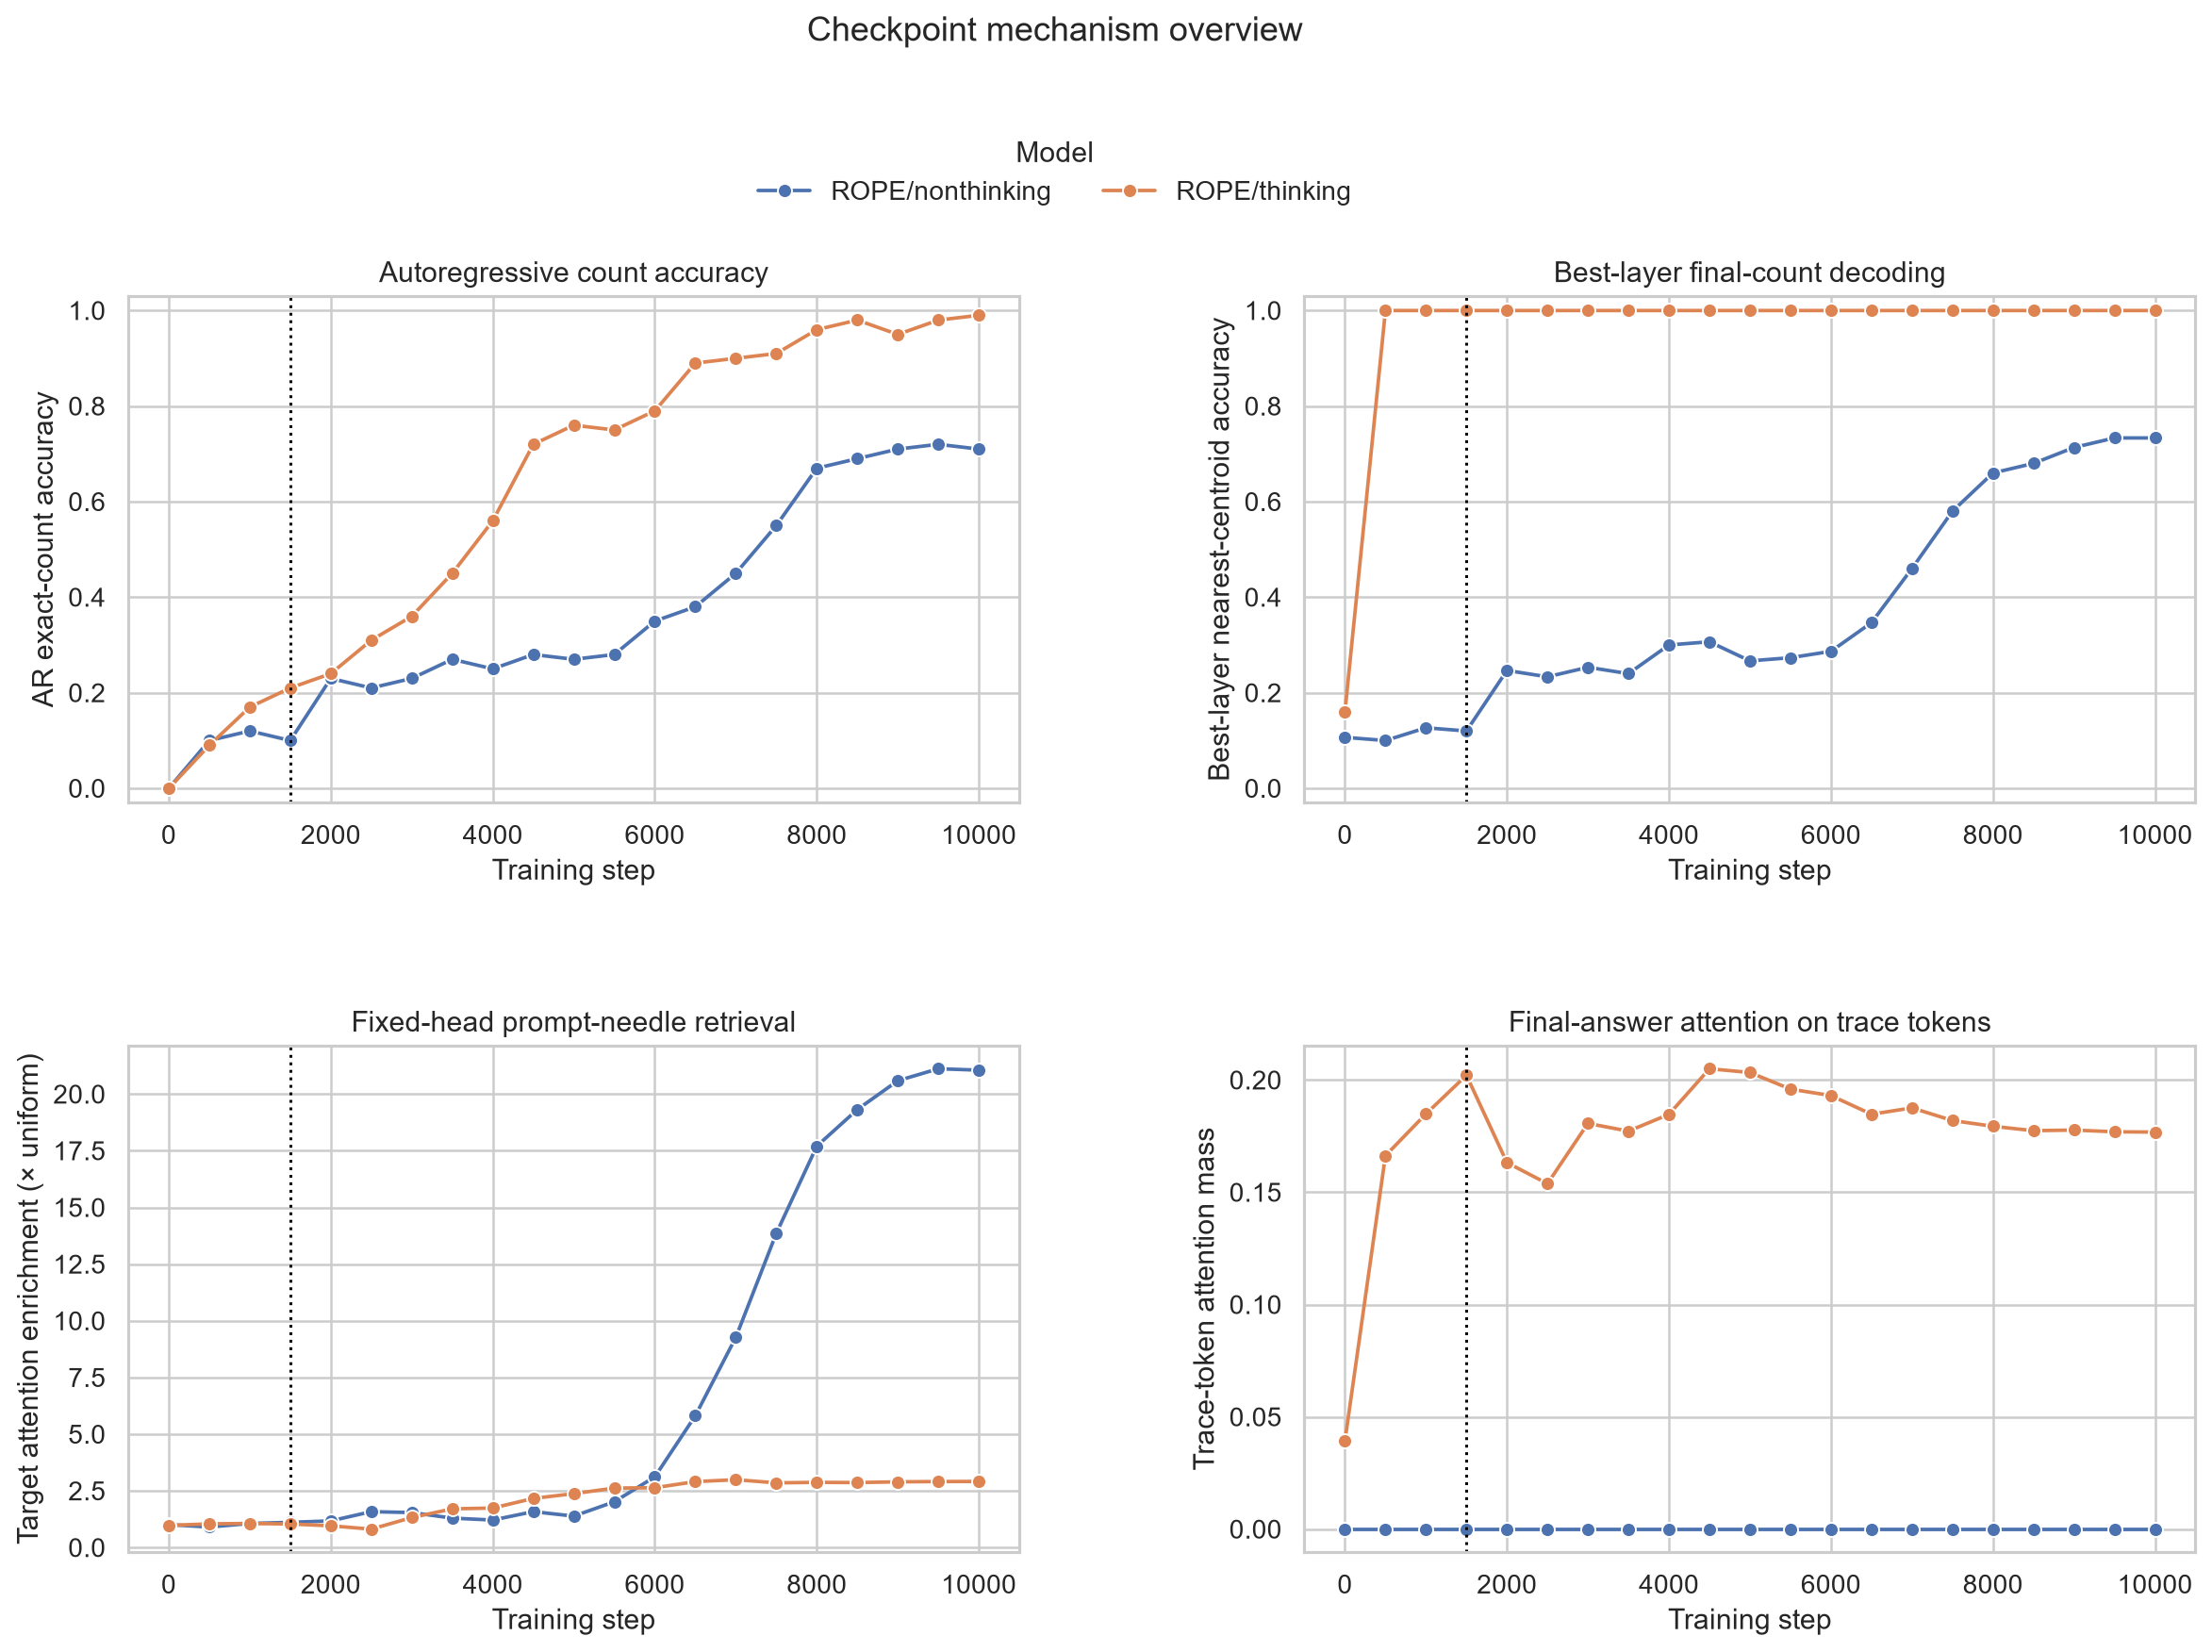
\includegraphics[width=\linewidth]{figures/synthetic_learning.png}
    \caption{Learning dynamics in the matched query-first run. Thinking forms a decodable final-answer state and answer-to-trace routing early; direct answering acquires broad prompt retrieval and high AR accuracy late. The dotted line marks the step-1,500 loss-scope switch.}
    \label{fig:learning}
\end{figure}

\subsection{The direct route aggregates broadly and writes count late}

At the final checkpoint, the strongest direct head (L4H2) covers 0.842 of the top-$n$ target occurrences and provides $21.1\times$ uniform target enrichment. This broad statistic is undefined for strict $k$-to-$k$ retrieval because direct answering has no $k$-indexed query.

The causal tests align with H-NT (Table~\ref{tab:causal}). Masking only the top broad head at \ans{} lowers accuracy from 82.5\% to 42.5\%; a matched random single head leaves 72.9\%. Patching the top four donor head slices into a receiver produces expected-count transport slope 0.680, versus 0.131 for random slices. Finally, an independently fitted adjacent-count centroid delta becomes nearly one-for-one executable only at Layer 4 (slope 0.958). Removing the first broad head also reduces downstream Layer-4 centroid accuracy from 75\% to 30\%, coupling the routing intervention to the predicted state damage.

\subsection{The trace route closes a serial causal loop}

Thinking exhibits distinct retrieval, progress, and readout components. The strongest held-out ordered-retrieval head has correct-top-1-minus-chance 0.467, while an early Layer-2 readout head places 0.873 attention mass on the trace. Count-preserving character corruption holds sequence length, total count, query location, and prefix set fixed. Restoring the top four clean targeted head slices recovers 0.909 of the marker margin, compared with 0.186 for a random ordering.

Successor/stop is also manipulable. At a position-matched marker query, the best head slice restores 0.801 of continue evidence in a close receiver and 0.488 in the reverse direction; the top four reach 0.930 and 0.911. MLP conversion is distributed: the top 16 of 1,024 Layer-4 features contain only 34.4\% of positive target-aligned evidence, while 256 features are needed for roughly 0.71 bidirectional recovery. A natural final-marker residual from a shorter trace, transplanted at the same absolute position, raises the close margin by 20.93 and causes 100\% of receivers to stop early.

The final scalar readout is separate from progress. Jointly ablating the two top readout heads only at \ans{} drops final accuracy from 100\% to 10\%, while random top-2 ablation leaves it at 100\%. Conversely, patching those two donor slices transports the full count with slope 1.000 (random: 0.024). Length-preserving replacements of the last trace pair---changing its index, marker, duplication, or content---leave the answer at $n$; physically deleting the pair moves \ans{} and flips all tested cases to $n-1$. A Layer-2 attention-output patch restores 0.998 of the clean margin. The strongest current conclusion is therefore that the readout exploits trace span or boundary position, not the identity of the final marker. RoPE distance and abstract pair count remain confounded.

Finally, residual state controls later routing. Replacing the pre-L3 progress state for receiver $k=3$ with donor progress $j=8$ increases L3H3 attention to the donor occurrence relative to the receiver occurrence by 0.338. Together with head-to-state damage, this supports a manipulable head $\rightarrow$ state $\rightarrow$ head loop rather than two correlated readouts.

\begin{table}[t]
\caption{Selected causal tests in the controlled query-first run. Random controls use matched deterministic head orderings; their min--max ranges are sanity checks, not confidence intervals.}
\label{tab:causal}
\centering
\small
\begin{tabular}{p{1.32in}p{1.40in}p{1.62in}}
\toprule
Route link & Intervention & Main result \\
\midrule
Direct heads $\rightarrow$ answer & query-local ablation & $82.5\%\rightarrow42.5\%$; random $72.9\%$ \\
Direct heads $\rightarrow$ count & donor head patch & top-4 slope $0.680$; random $0.131$ \\
Direct state $\rightarrow$ count & centroid steering & L4 slope $0.958$ \\
Targeted heads $\rightarrow M_k$ & clean head patch & top-4 recovery $0.909$; random $0.186$ \\
Readout heads $\rightarrow C_n$ & query-local ablation & $100\%\rightarrow10\%$; random $100\%$ \\
Readout heads $\rightarrow C_n$ & donor head patch & top-2 slope $1.000$; random $0.024$ \\
Final marker $\rightarrow$ stop & residual transplant & close shift $+20.93$; $100\%$ stop \\
Progress $\rightarrow$ routing & residual transplant & donor-relative mass shift $+0.338$ \\
\bottomrule
\end{tabular}
\end{table}

\section{Query placement rewires the route}
\label{sec:layout}

Moving the query after the data improves direct counting substantially (Table~\ref{tab:layout}; Figure~\ref{fig:layout}). On 100 paired AR prompts, accuracy rises from 84\% to 96\% (paired bootstrap 95\% CI $[+6,+19]$ points; 12 fixes and no regressions). The diagnostic accuracy area under the learning curve rises from 0.361 to 0.694, and persistent 80\% accuracy moves from unreached to step 4,500. Thinking final answers are ceiling-limited (98\% to 99\%), but exact traces improve from 81\% to 98\%.

The internal route changes, not merely the score. Under query-first, direct answering ends with strong data coverage (top-$n$ recall 0.842) and weak answer-to-query routing. Under query-last, direct data coverage falls to 0.074 while an L2 answer head puts 0.963 mass on the five nearby query tokens. Direct final-answer count becomes decodable much earlier: Layer-2 $R^2$ rises from 0.550 to 0.978, with centroid accuracy from 0.140 to 0.873. These four observations---behavior, learning time, head role, and state location---support a data $\rightarrow$ query $\rightarrow$ answer bottleneck. The data-to-query arrow remains a hypothesis because query-site states and patches have not yet been measured.

\begin{table}[t]
\caption{Paired query-first versus query-last outcomes. The bootstrap interval reflects finite evaluation prompts, not training-seed variance.}
\label{tab:layout}
\centering
\small
\begin{tabular}{lccc}
\toprule
Metric & Query-first & Query-last & Difference \\
\midrule
Direct TF accuracy ($N=500$) & 79.4\% & 95.2\% & $+15.8$ pp \\
Direct AR accuracy ($N=100$) & 84.0\% & 96.0\% & $+12.0$ pp \\
Thinking AR accuracy ($N=100$) & 98.0\% & 99.0\% & $+1.0$ pp \\
Thinking exact trace ($N=100$) & 81.0\% & 98.0\% & $+17.0$ pp \\
Direct L2 count $R^2$ & 0.550 & 0.978 & $+0.428$ \\
\bottomrule
\end{tabular}
\end{table}

\begin{figure}[t]
    \centering
    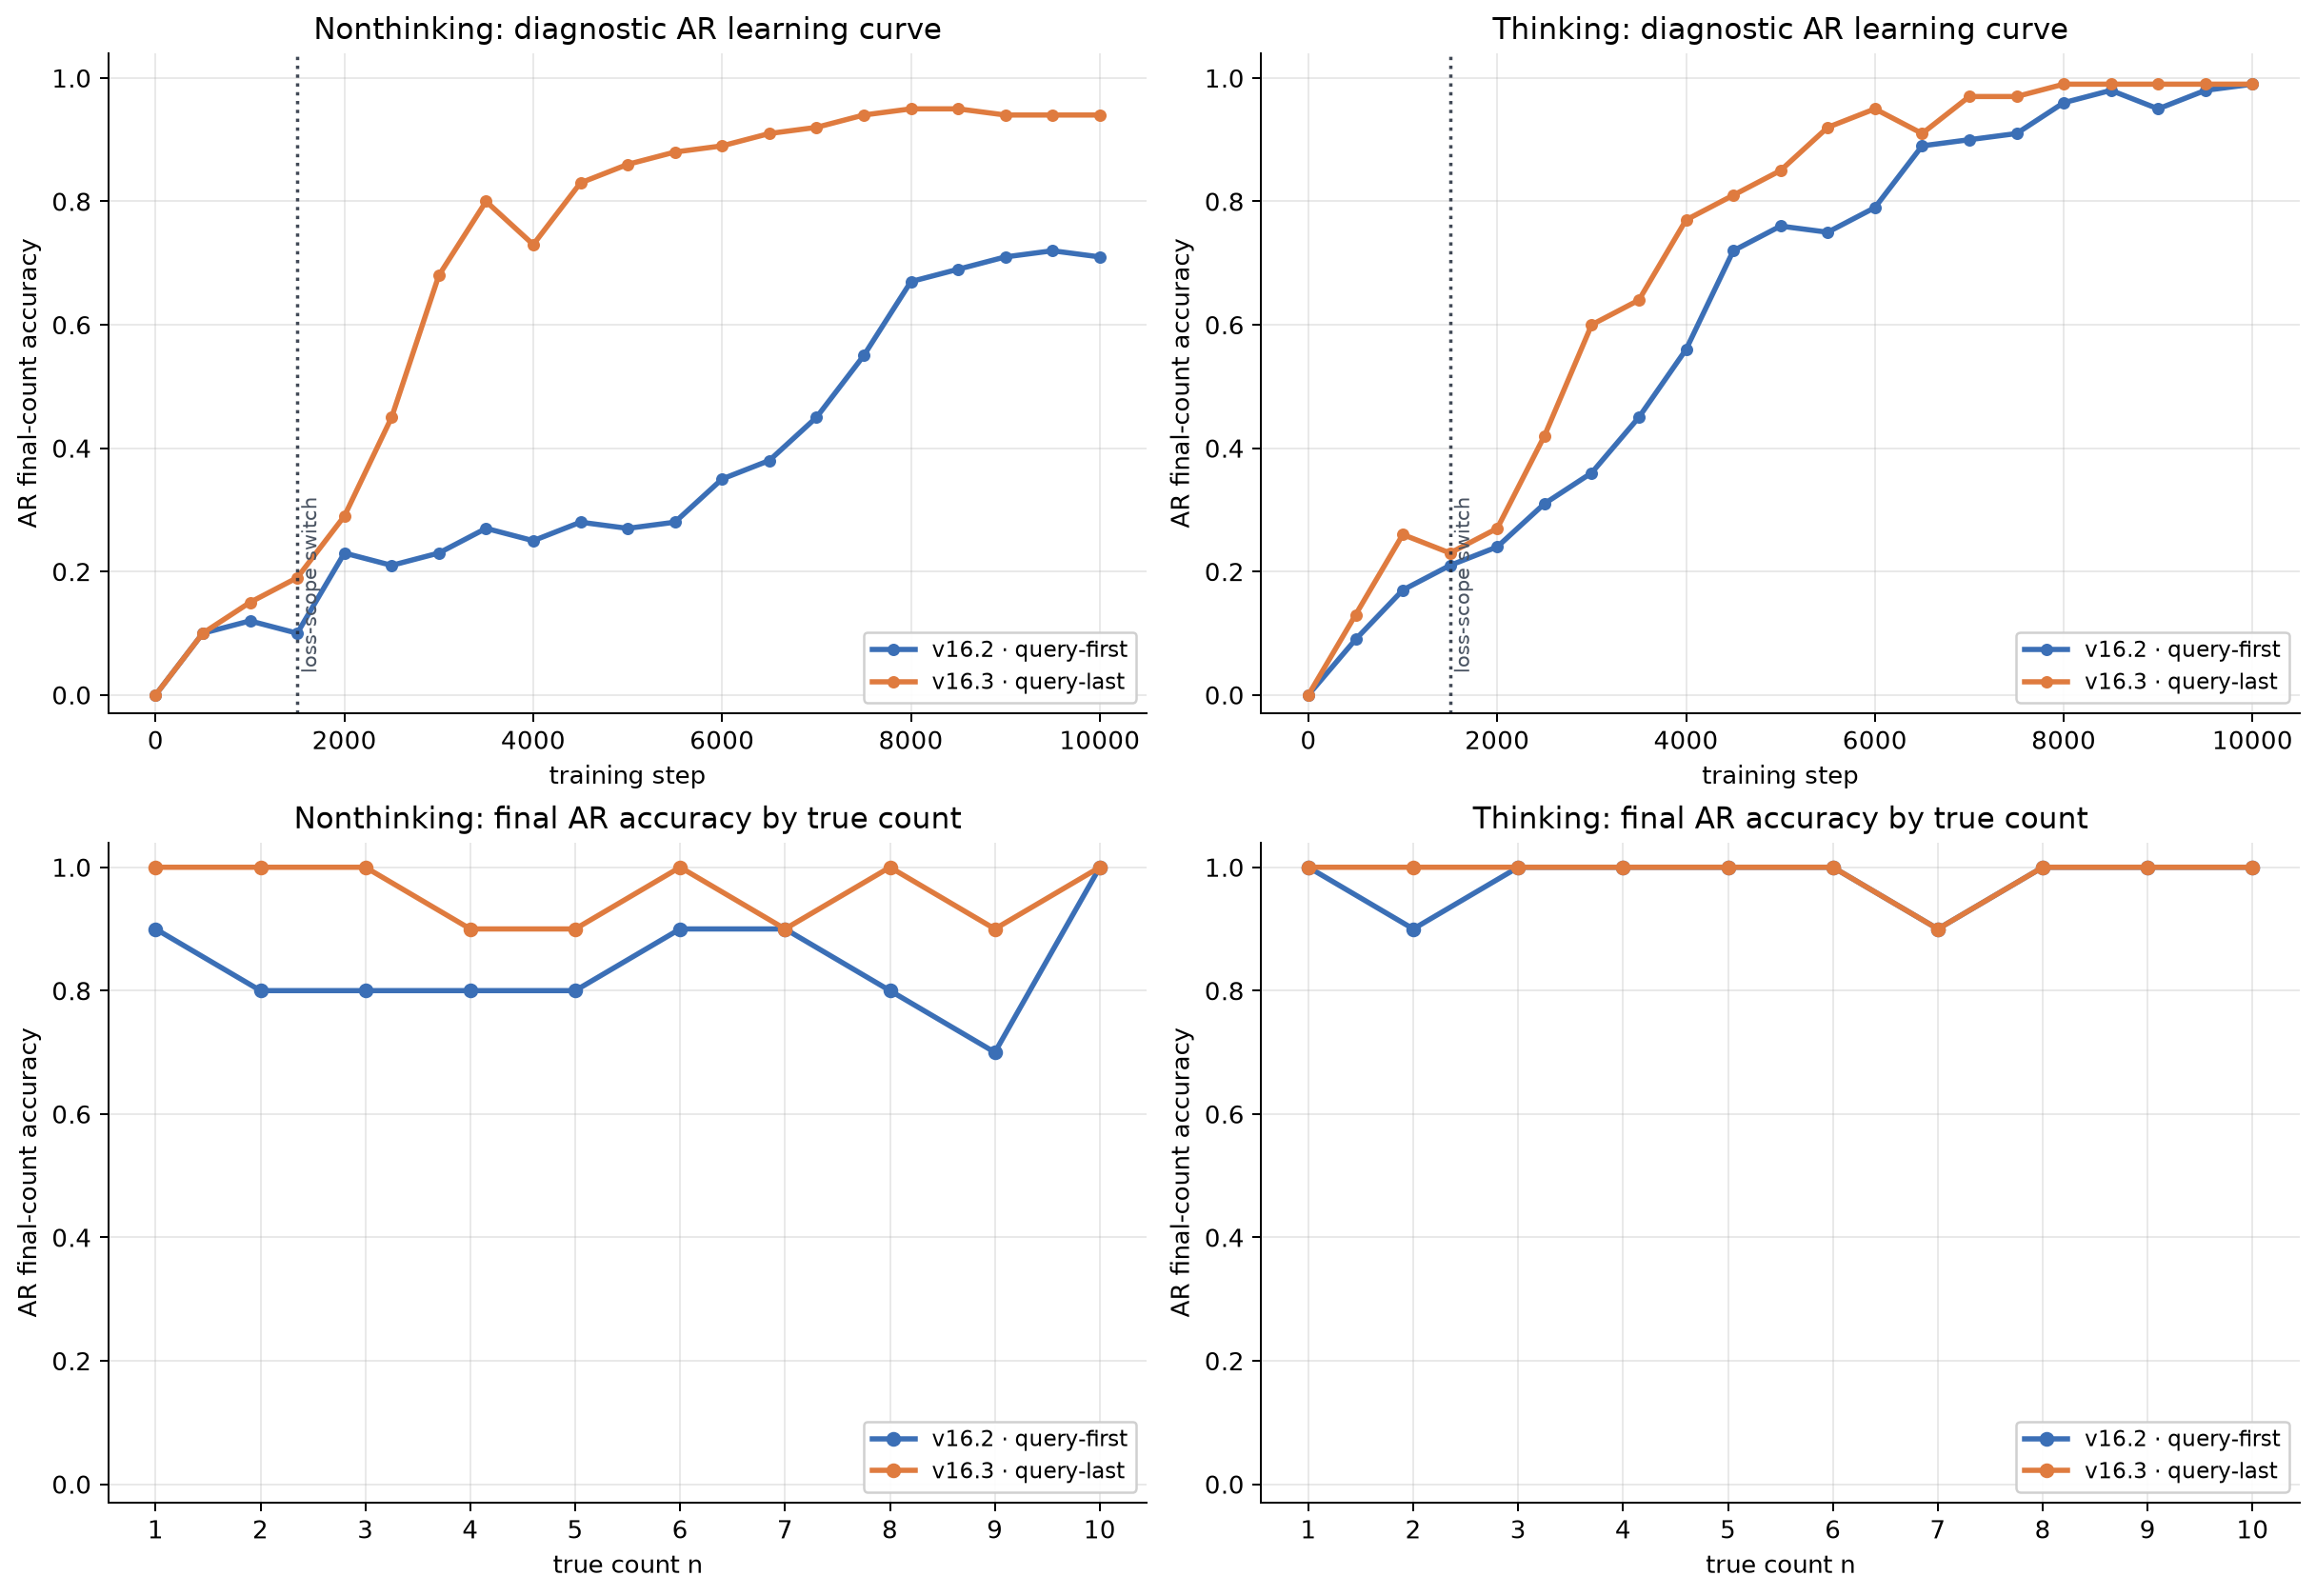
\includegraphics[width=\linewidth]{figures/query_order_behavior.png}
    \caption{Query placement intervention. Top: checkpoint diagnostic AR accuracy. Bottom: independent final accuracy by count (10 examples per count). Query-last particularly accelerates and improves direct counting; thinking is near the final-answer ceiling in both layouts.}
    \label{fig:layout}
\end{figure}

\section{Realistic long-context counting}
\label{sec:realistic}

\subsection{Retrieval succeeds where aggregation fails}

The realistic models sharply dissociate retrieval from counting. In the list condition, both models recall at least 94\% of inserted records; Qwen remains near 100\% even at $N=40$. Bare Qwen counting is 80--100\% for $N\leq3$ but falls to 7\% at $N=4$ and becomes dominated by integer attractors thereafter (Figure~\ref{fig:realistic}a). In a stronger within-trial control, Qwen produces both ``count $\mid$ first city'' in one forward generation: first-city recall is 0.99--1.00 for $N\in\{5,10,15,20,30\}$, while the count is 0.00--0.01. The failure is therefore not adequately explained by losing the needles in the middle \citep{liu2024lost}; the model finds an item but fails to aggregate all items.

\subsection{Enumeration supplies the missing interface}

Requiring a list before the total improves both architectures (Figure~\ref{fig:realistic}b). For Qwen, unnumbered enumeration raises accuracy at $N=20$ from about 0.22 to 0.84; for Olmo-Hybrid it raises accuracy at $N=20$ from about 0.03 to 0.22. The unnumbered scaffold itself eventually saturates, but explicit numbered enumeration turns the task into retrieving the last index and reaches 0.97 accuracy at $N=40$. A placement control shows that an identical gold list is much more useful when it appears as assistant-side context immediately before generation than when separated from the answer by the user question (0.87 versus 0.37 at $N=20$). Thus list structure and causal location, not a privileged act of self-generation, are the active ingredients.

\begin{figure}[t]
    \centering
    \begin{minipage}[t]{0.49\linewidth}
        \centering
        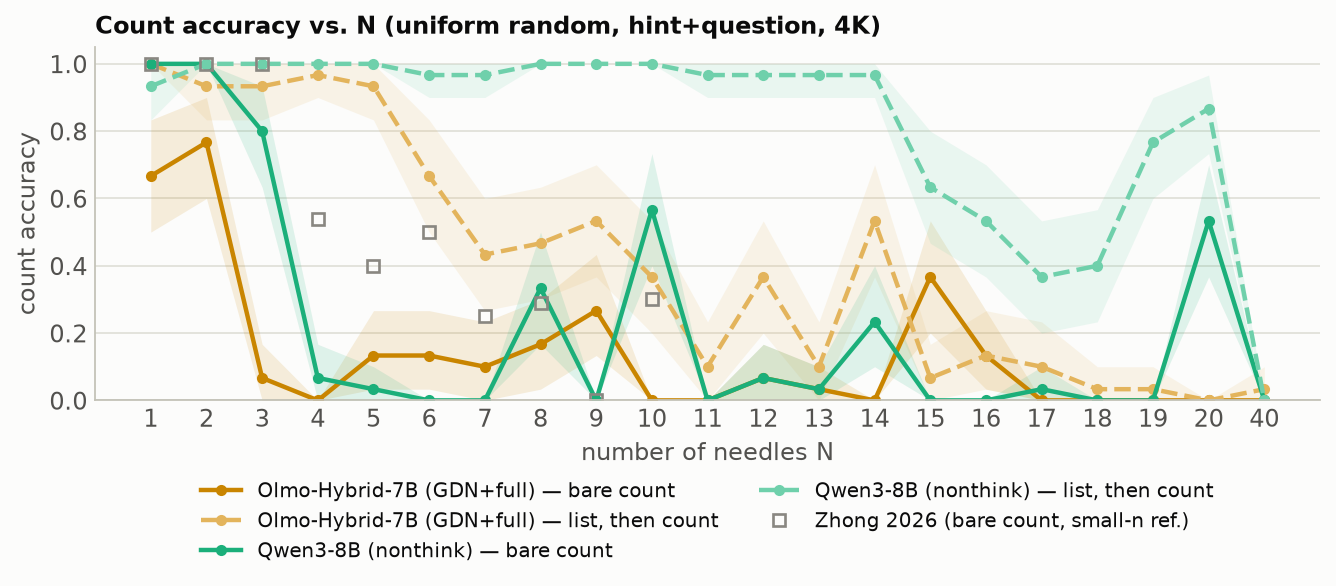
\includegraphics[width=\linewidth]{figures/realistic_count_curve.png}\\[-1mm]
        \small (a) Bare and enumerated accuracy across $N$.
    \end{minipage}\hfill
    \begin{minipage}[t]{0.49\linewidth}
        \centering
        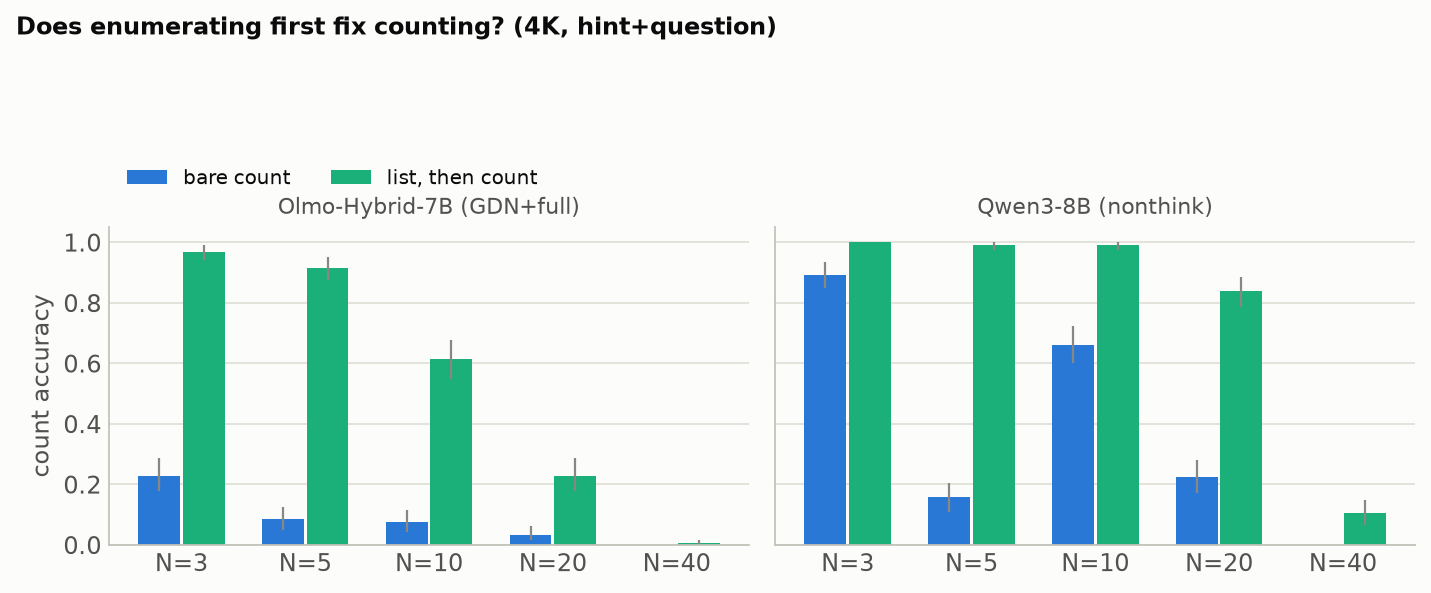
\includegraphics[width=\linewidth]{figures/realistic_enumeration_scaffold.png}\\[-1mm]
        \small (b) Paired enumeration effect at main counts.
    \end{minipage}
    \caption{Realistic 4K NIAH. Bare counting collapses well before item retrieval does; enumerating records before producing the total restores substantial accuracy. Error bars and bands are 95\% intervals over independently generated prompts.}
    \label{fig:realistic}
\end{figure}

\subsection{Mechanistic correspondence at scale}

Qwen's bare-count mechanism maps to H-NT at a coarser scale. Adding filler at fixed $N$ monotonically lowers the estimate even though 8K item recall remains 1.0. At the readout token, a small head family attends nearly uniformly over all needles; total needle mass saturates while per-needle mass falls approximately as $1/N$. No linear or MLP probe recovers a running count from states between needles after controlling for depth, but the final-token magnitude state is manipulable: steering along its probe direction moves the output with slope 0.65 while preserving lattice quantization. Aggregator-head ablation roughly halves accuracy. These observations support a delayed parallel proportion code rather than a robust sequential counter.

The explicit-trace runs provide complementary, though less complete, evidence for H-CoT. Without CoT, answer-site attention is broad and noisy; at numbered trace spans, middle/high-layer heads attend to one prompt record at a time in order. Prompt and CoT span probes reach test $R^2=0.979$ and $0.987$, respectively, but their directions are nearly orthogonal and naive steering is weak. This is precisely why the controlled causal battery is necessary: decodability alone does not establish which state the model reads out.

\section{Related work}

\paragraph{Intermediate computation.}
Scratchpads and CoT improve multi-step reasoning by externalizing intermediate states \citep{nye2021scratchpads,wei2022cot}. Filler tokens can also provide useful compute \citep{pfau2024dot}, and program-like traces can support length generalization \citep{hou2025turing}. Our result is more specific: for counting, semantically aligned index--marker pairs create addressable retrieval, progress, and readout sites. The query-layout intervention further shows that interface placement can change the learned route at fixed output position.

\paragraph{Counting in transformers.}
Prior work studies algorithmic generalization and representational limits of counting \citep{ouellette2023counting,yehudai2024count}. Mechanistic studies find linearly decodable or transferable internal count states \citep{hasani2025counting,garcia2026wrong}. We reconcile strong probes with poor behavior by separating representation from routing: count or ordinal information may exist at item sites yet fail to reach the answer. Our direct route is also consistent with a geometric readout bottleneck, while our trace route demonstrates that changing the output interface can construct a different causal path rather than merely rotate one count vector.

\paragraph{Long-context retrieval and aggregation.}
Long-context performance depends on item position \citep{liu2024lost}, while RULER shows that retrieval and aggregation must be evaluated separately \citep{hsieh2024ruler}. Our realistic experiments make this separation within matched prompts and even within a single generated response. They then connect the behavioral gap to attention dilution, residual geometry, and causal interventions.

\section{Limitations and conclusion}

The controlled comparison has one training seed, one small 4-layer architecture, one character corpus, and counts 1--10. Head identities may permute or split across seeds; role-level replication is required. The query-last comparison jointly changes causal visibility, RoPE distance, and data positions, and its proposed query bottleneck lacks direct query-site patching. The strongest trace readout result still confounds abstract trace length with RoPE-relative boundary position. Several patches use teacher-forced or constructed corruptions rather than naturally occurring AR failures. In the realistic study, mechanistic depth is greatest for Qwen3-8B, while Olmo-Hybrid mainly provides behavioral architecture contrast; model and context-length coverage should expand. Finally, a supervised indexed trace is an idealized form of CoT and should not be conflated with free-form natural-language explanations.

Within these boundaries, the results support a simple answer to the motivating question. A transformer can count directly by broadly aggregating a set into a late scalar state, but this path is late-learning and susceptible to dilution and readout mismatch. An explicit trace creates a serial workspace with stable addresses: each step retrieves one item, updates progress, and leaves a structure that the answer query can read. CoT helps counting here because it changes the computation's interface and route, not because it merely reveals a better linear number representation.

\paragraph{Ethics statement.}
This work uses synthetic character sequences and publicly available essay text to study model internals. It does not involve human subjects or private data. Mechanistic methods may improve auditing but can also enable targeted model manipulation; we report interventions and limitations to support reproducibility and responsible interpretation.

\section*{Acknowledgments}
\todo{Add acknowledgments, funding sources, compute credits, and any required disclosure statements.}

\bibliography{references}
\bibliographystyle{plainnat}

\appendix

\section{Exact sequence formats and metrics}

For a target set $S$ of three characters and data window $x_{1:256}$, the query-first nonthinking sequence is schematically
\begin{equation*}
\texttt{<BOS> <CountChar> } S \texttt{ <Sep> } x_{1:256}
\texttt{ <Ans> } C_n \texttt{ <EOS>}.
\end{equation*}
The thinking sequence shares the prefix and appends
\begin{equation*}
\think{}\; \texttt{<1>}M_1\cdots\texttt{<n>}M_n\;\close{}\;\ans{}\;C_n\;\texttt{<EOS>}.
\end{equation*}
The query-last condition swaps the positions of the query and $x_{1:256}$ but keeps the output starting at position 262.

For a head with attention $a(q,p)$ and target positions $P$, target mass is $\sum_{p\in P}a(q,p)$. Broad coverage also reports target-normalized entropy and top-$n$ target recall. Ordered retrieval reports whether $p_k$ is top-1 among $P$ at the $k$th trace index, minus chance $1/n$. Expected-count transport is the through-origin slope of the patched expected count against donor offset $m-n$, using a softmax restricted to count tokens. A slope of 1 denotes one-for-one transport.

\clearpage
\section{Additional controlled results}

\begin{figure}[h]
    \centering
    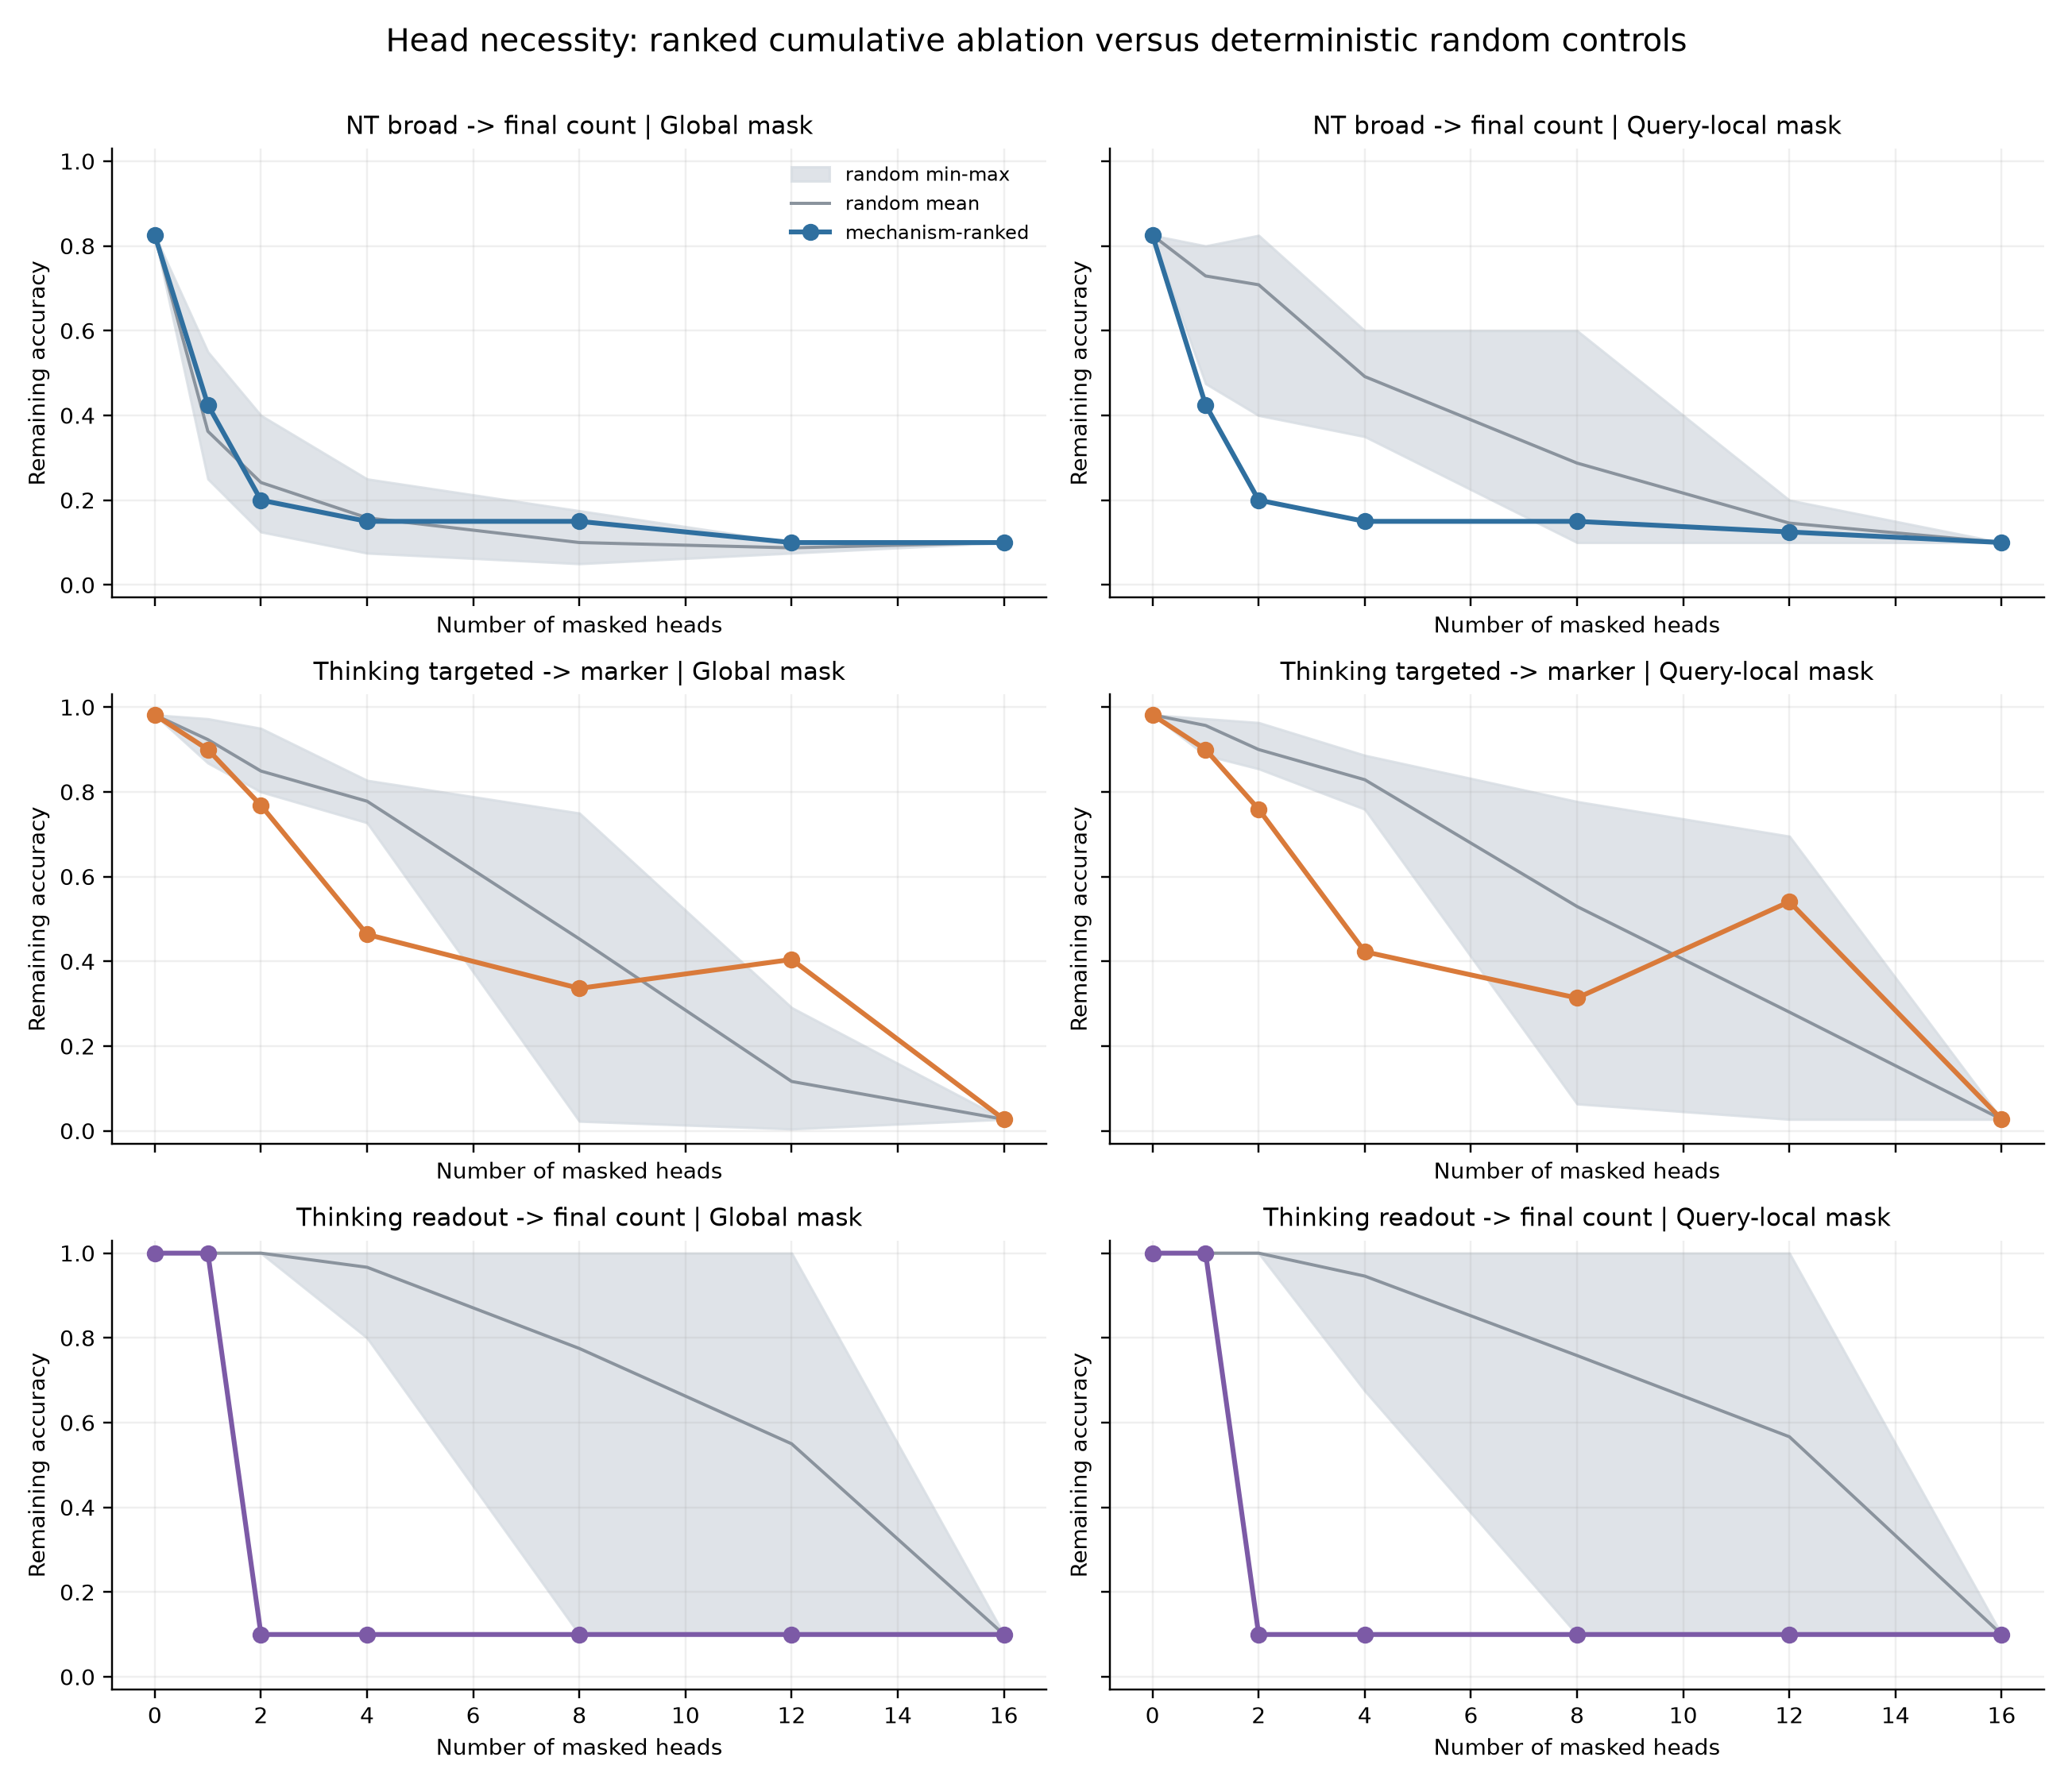
\includegraphics[width=\linewidth]{figures/synthetic_ablation.png}
    \caption{Global and query-local cumulative head ablation for direct broad aggregation, trace targeted retrieval, and trace readout. Mechanism-ranked paths are compared with six deterministic random paths.}
    \label{fig:app-ablation}
\end{figure}

\begin{figure}[h]
    \centering
    \begin{minipage}[t]{0.49\linewidth}
        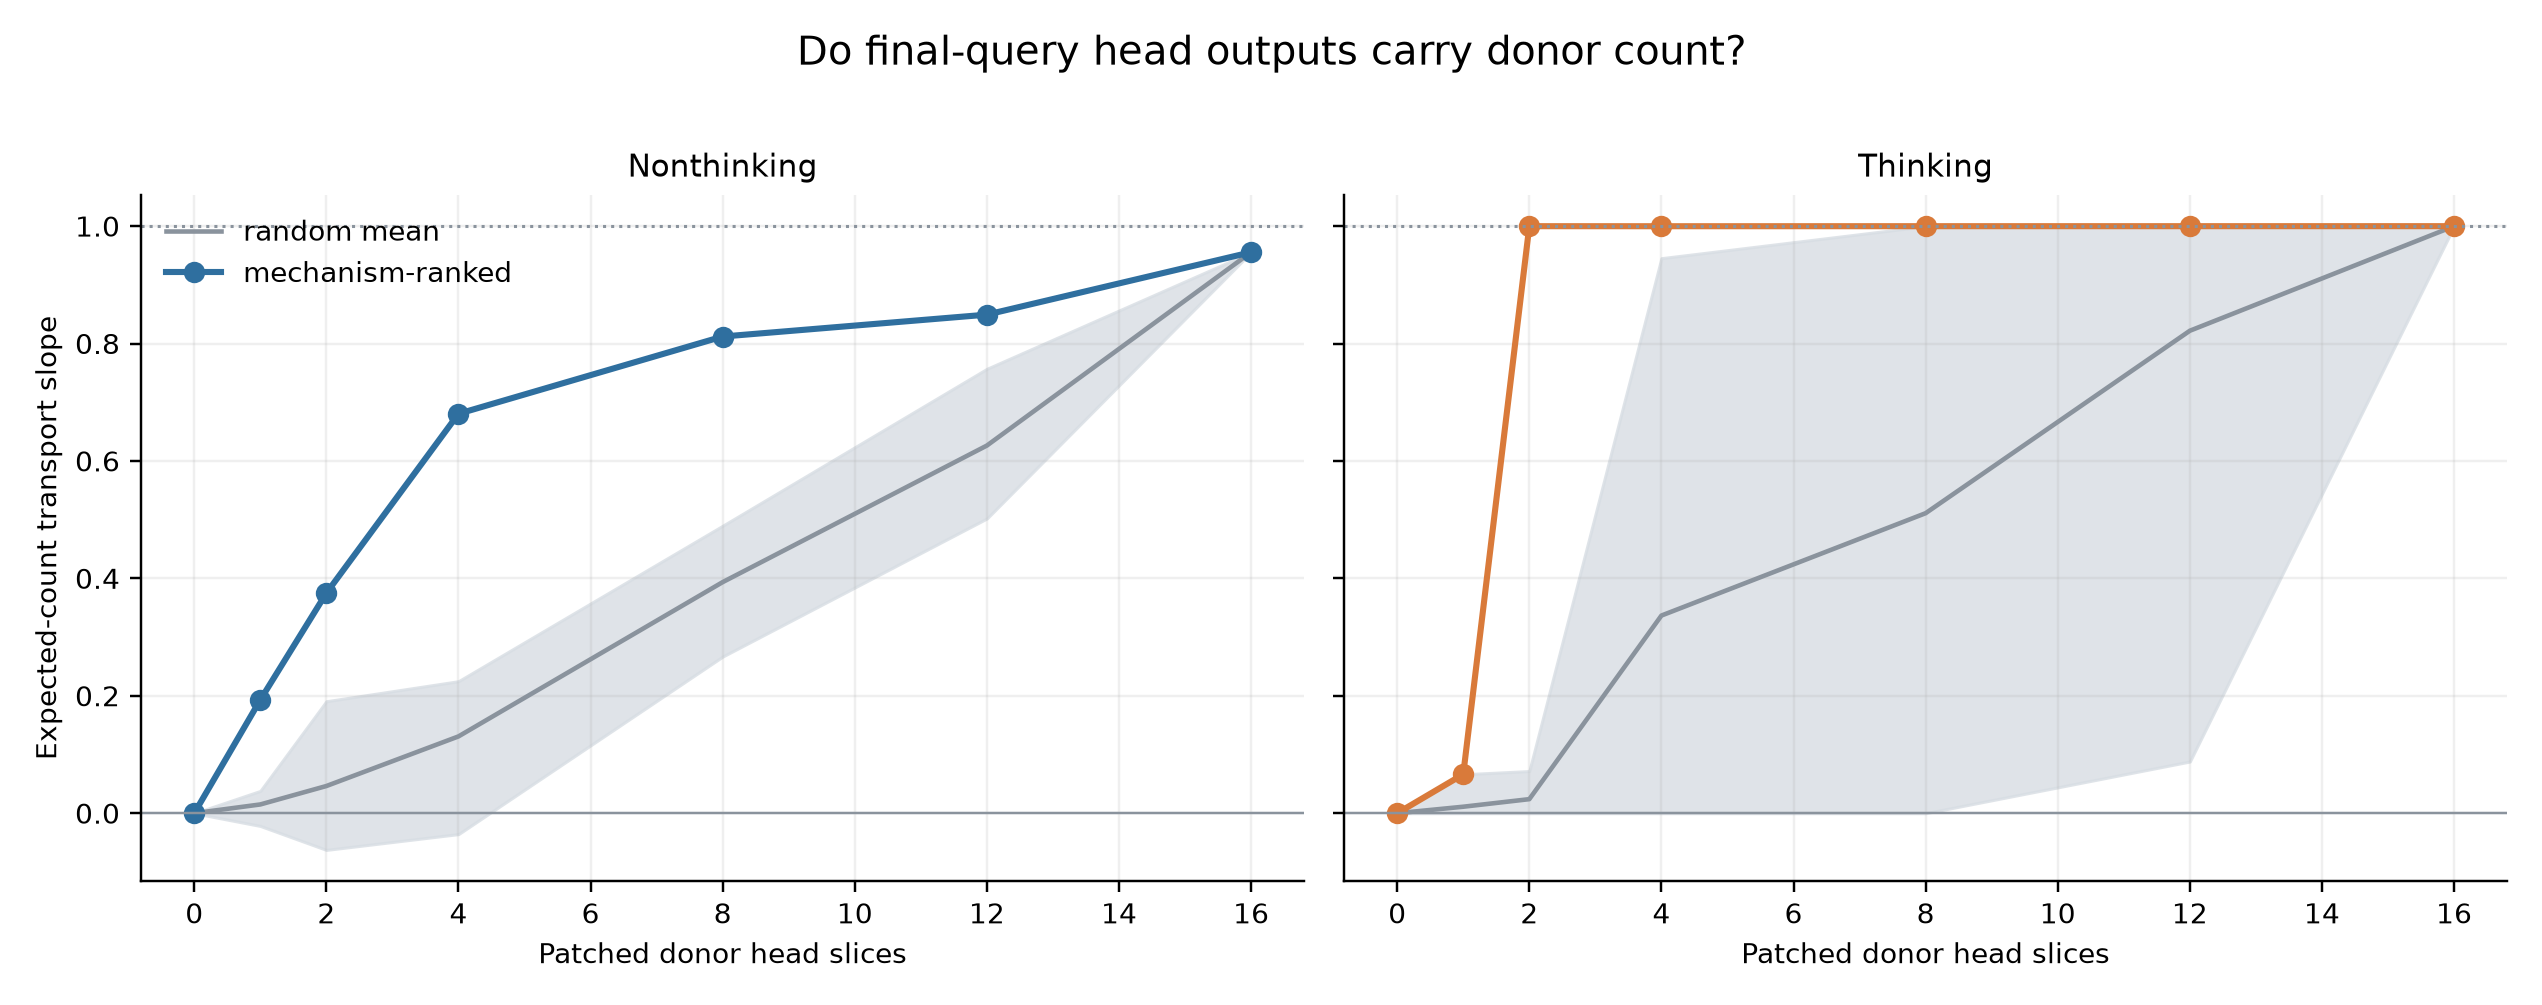
\includegraphics[width=\linewidth]{figures/synthetic_transport.png}
    \end{minipage}\hfill
    \begin{minipage}[t]{0.49\linewidth}
        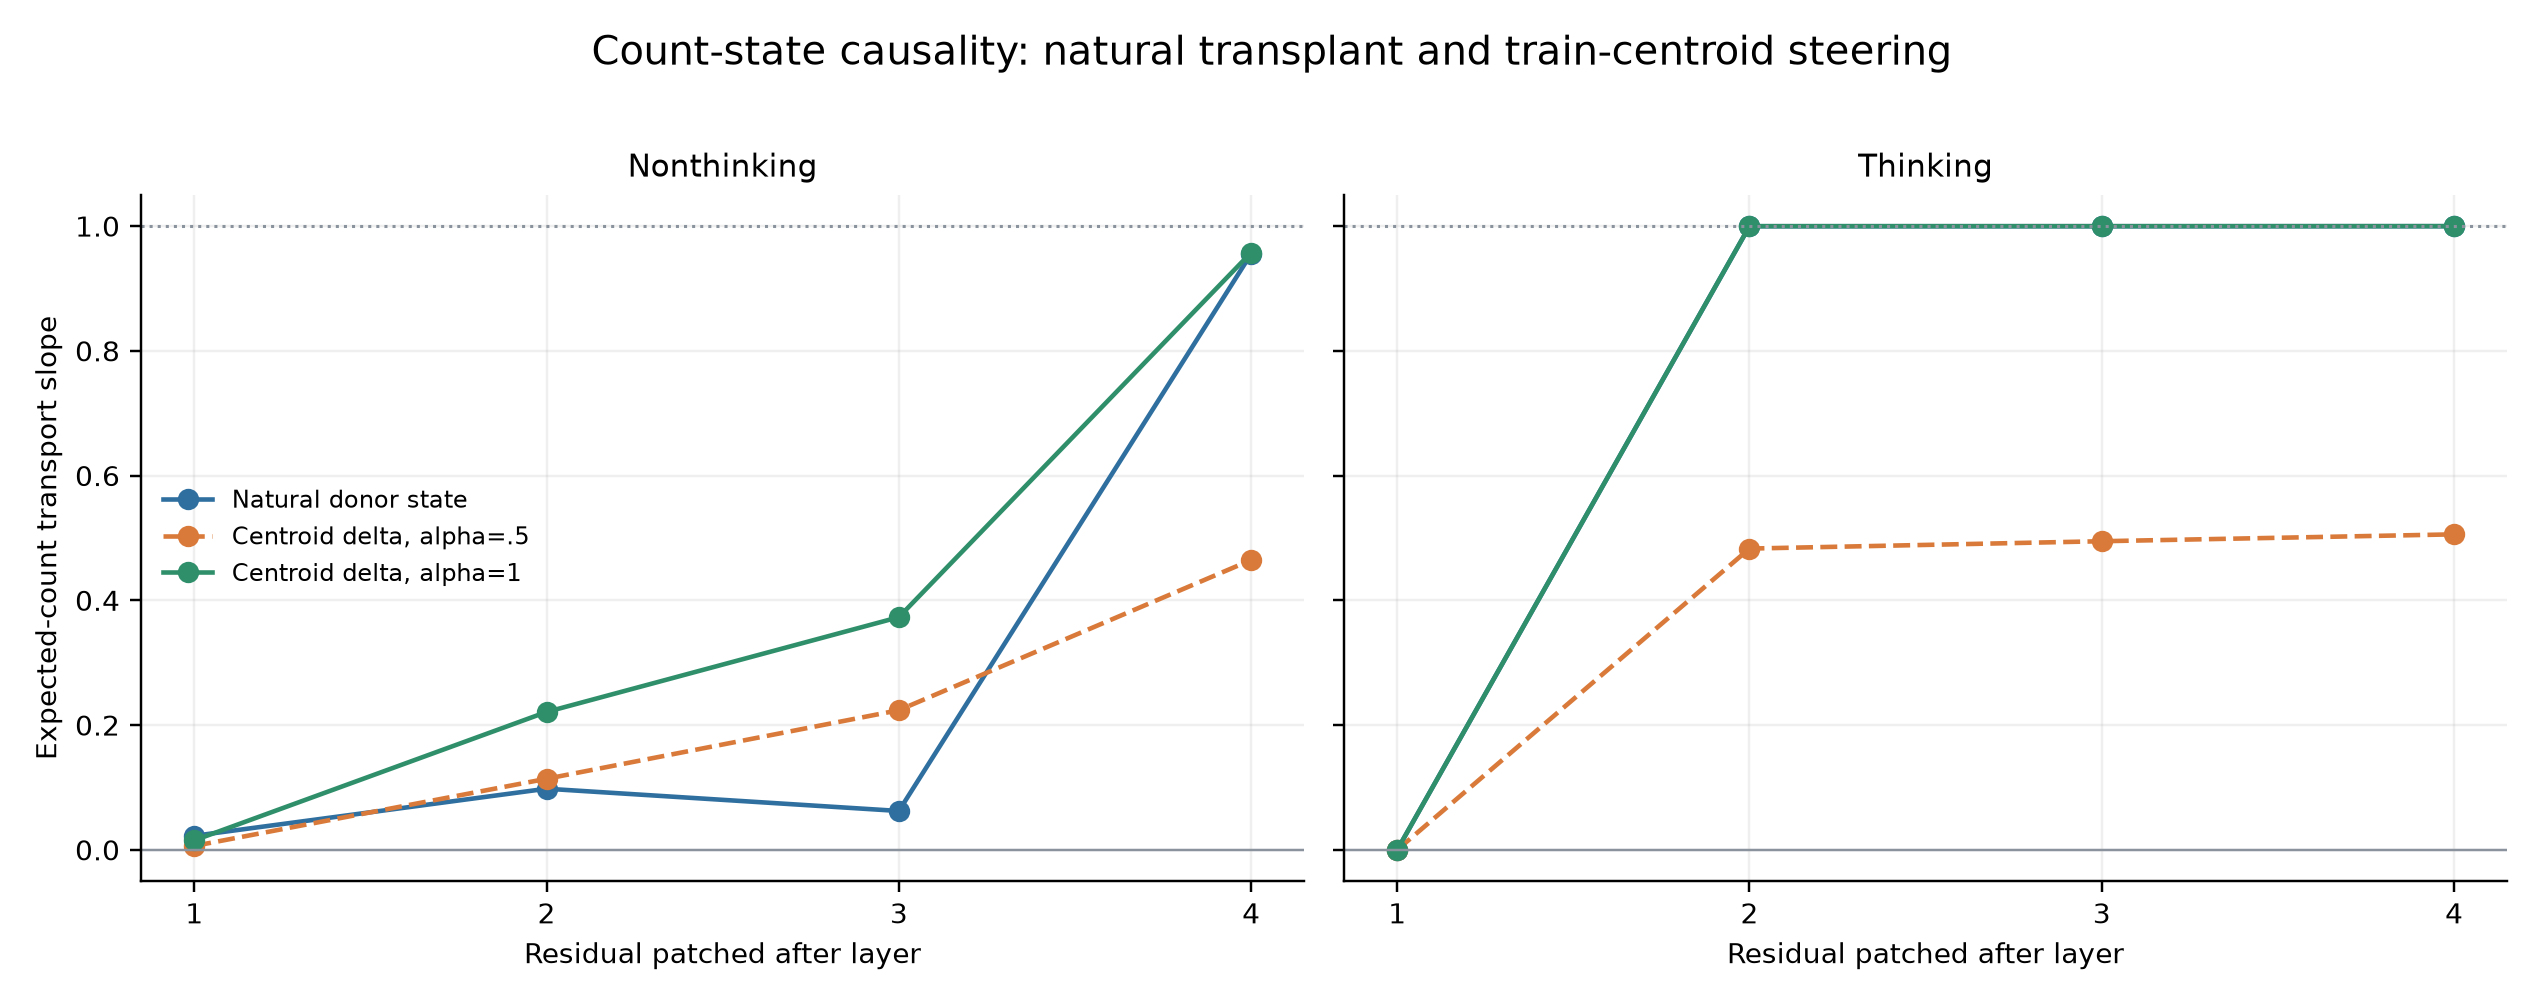
\includegraphics[width=\linewidth]{figures/synthetic_steering.png}
    \end{minipage}
    \caption{Left: donor-count transport through answer-query head slices. Right: natural residual transplant and independently fitted centroid steering.}
    \label{fig:app-transport}
\end{figure}

\begin{figure}[h]
    \centering
    \begin{minipage}[t]{0.49\linewidth}
        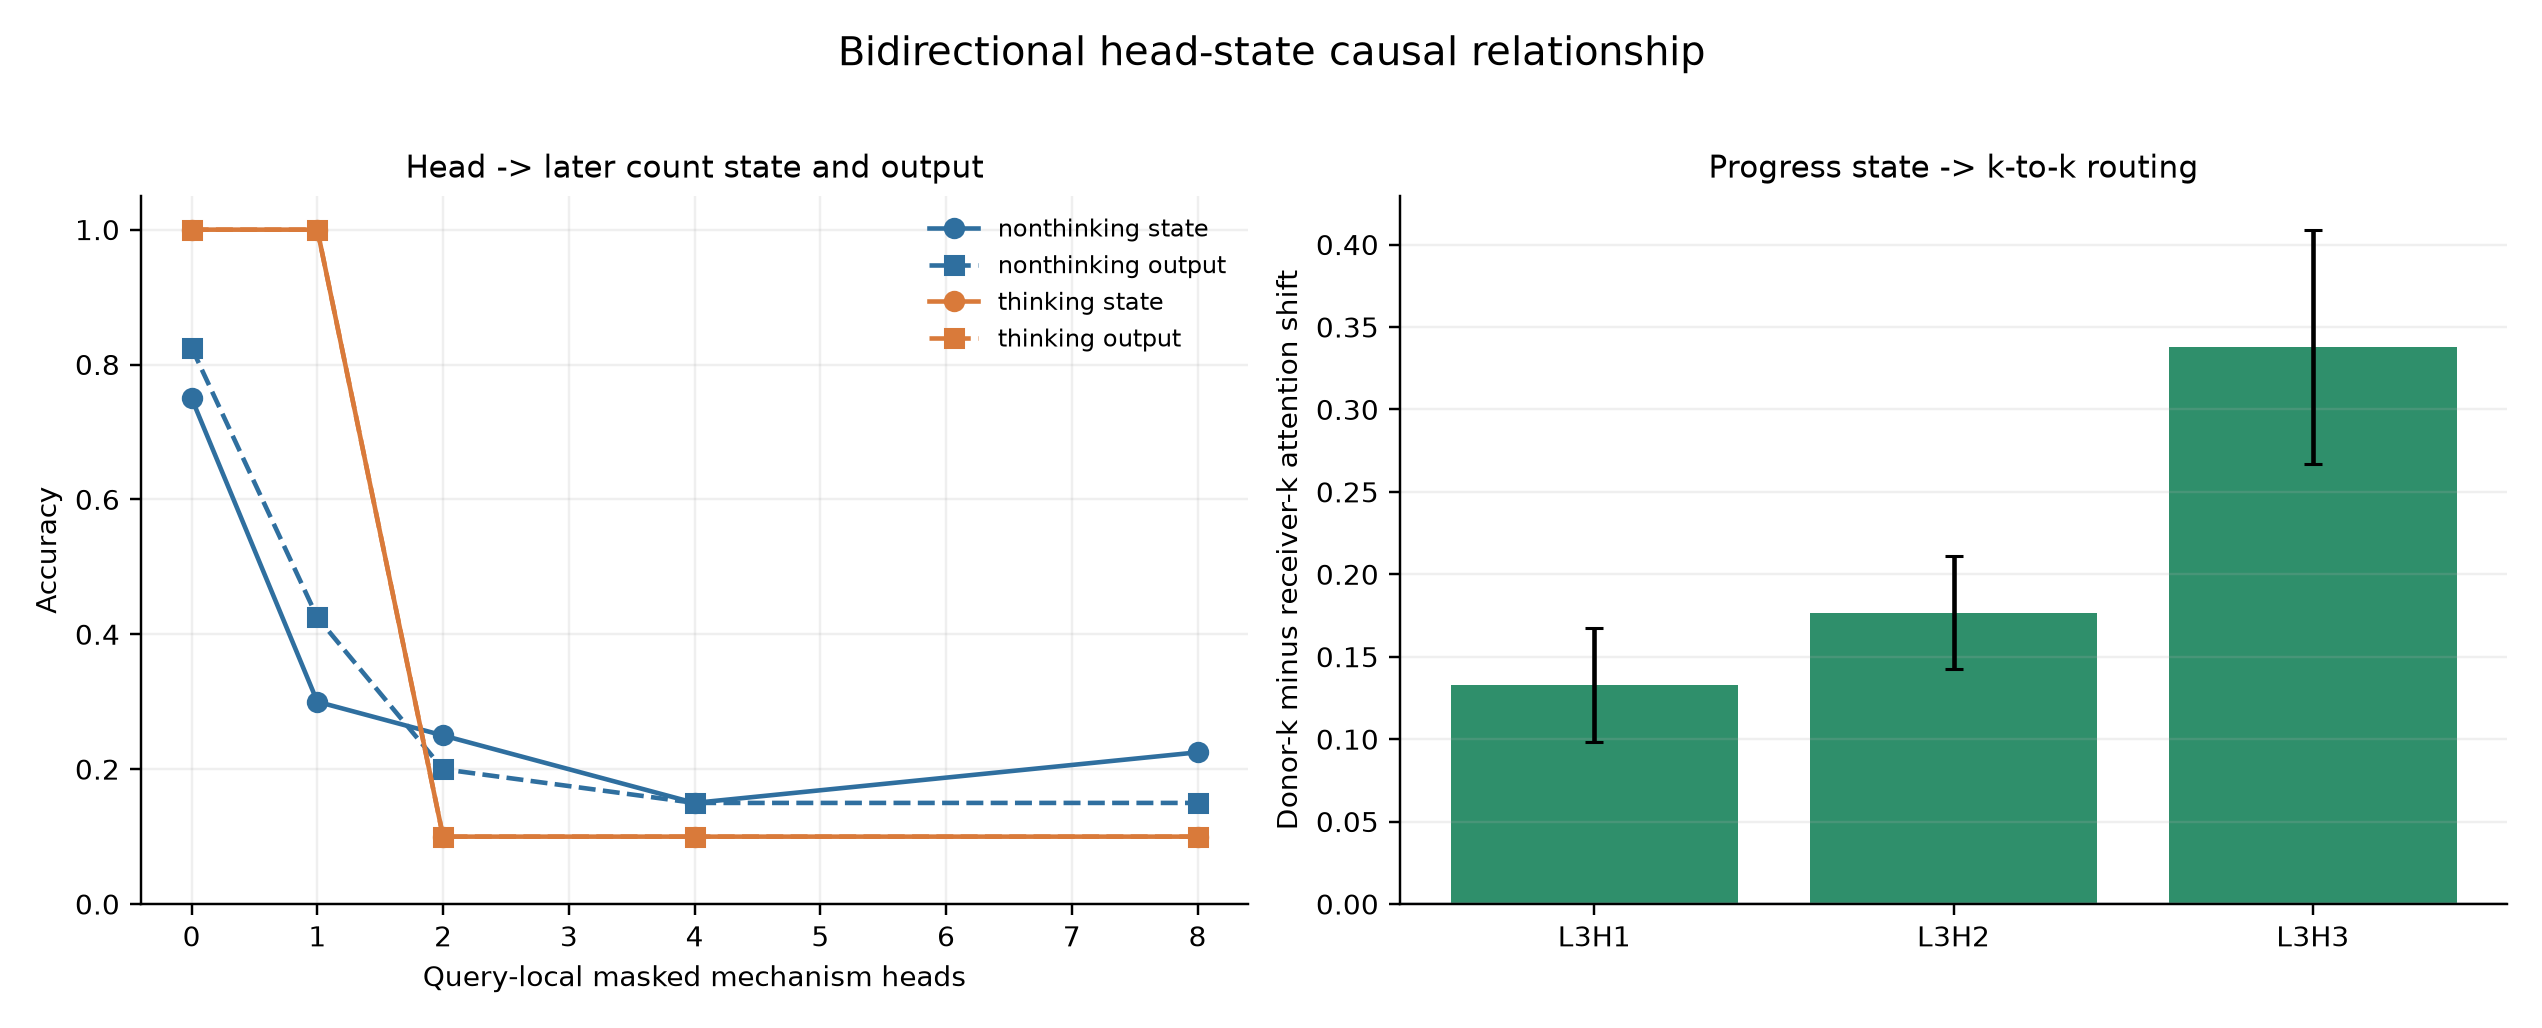
\includegraphics[width=\linewidth]{figures/synthetic_head_state_loop.png}
    \end{minipage}\hfill
    \begin{minipage}[t]{0.49\linewidth}
        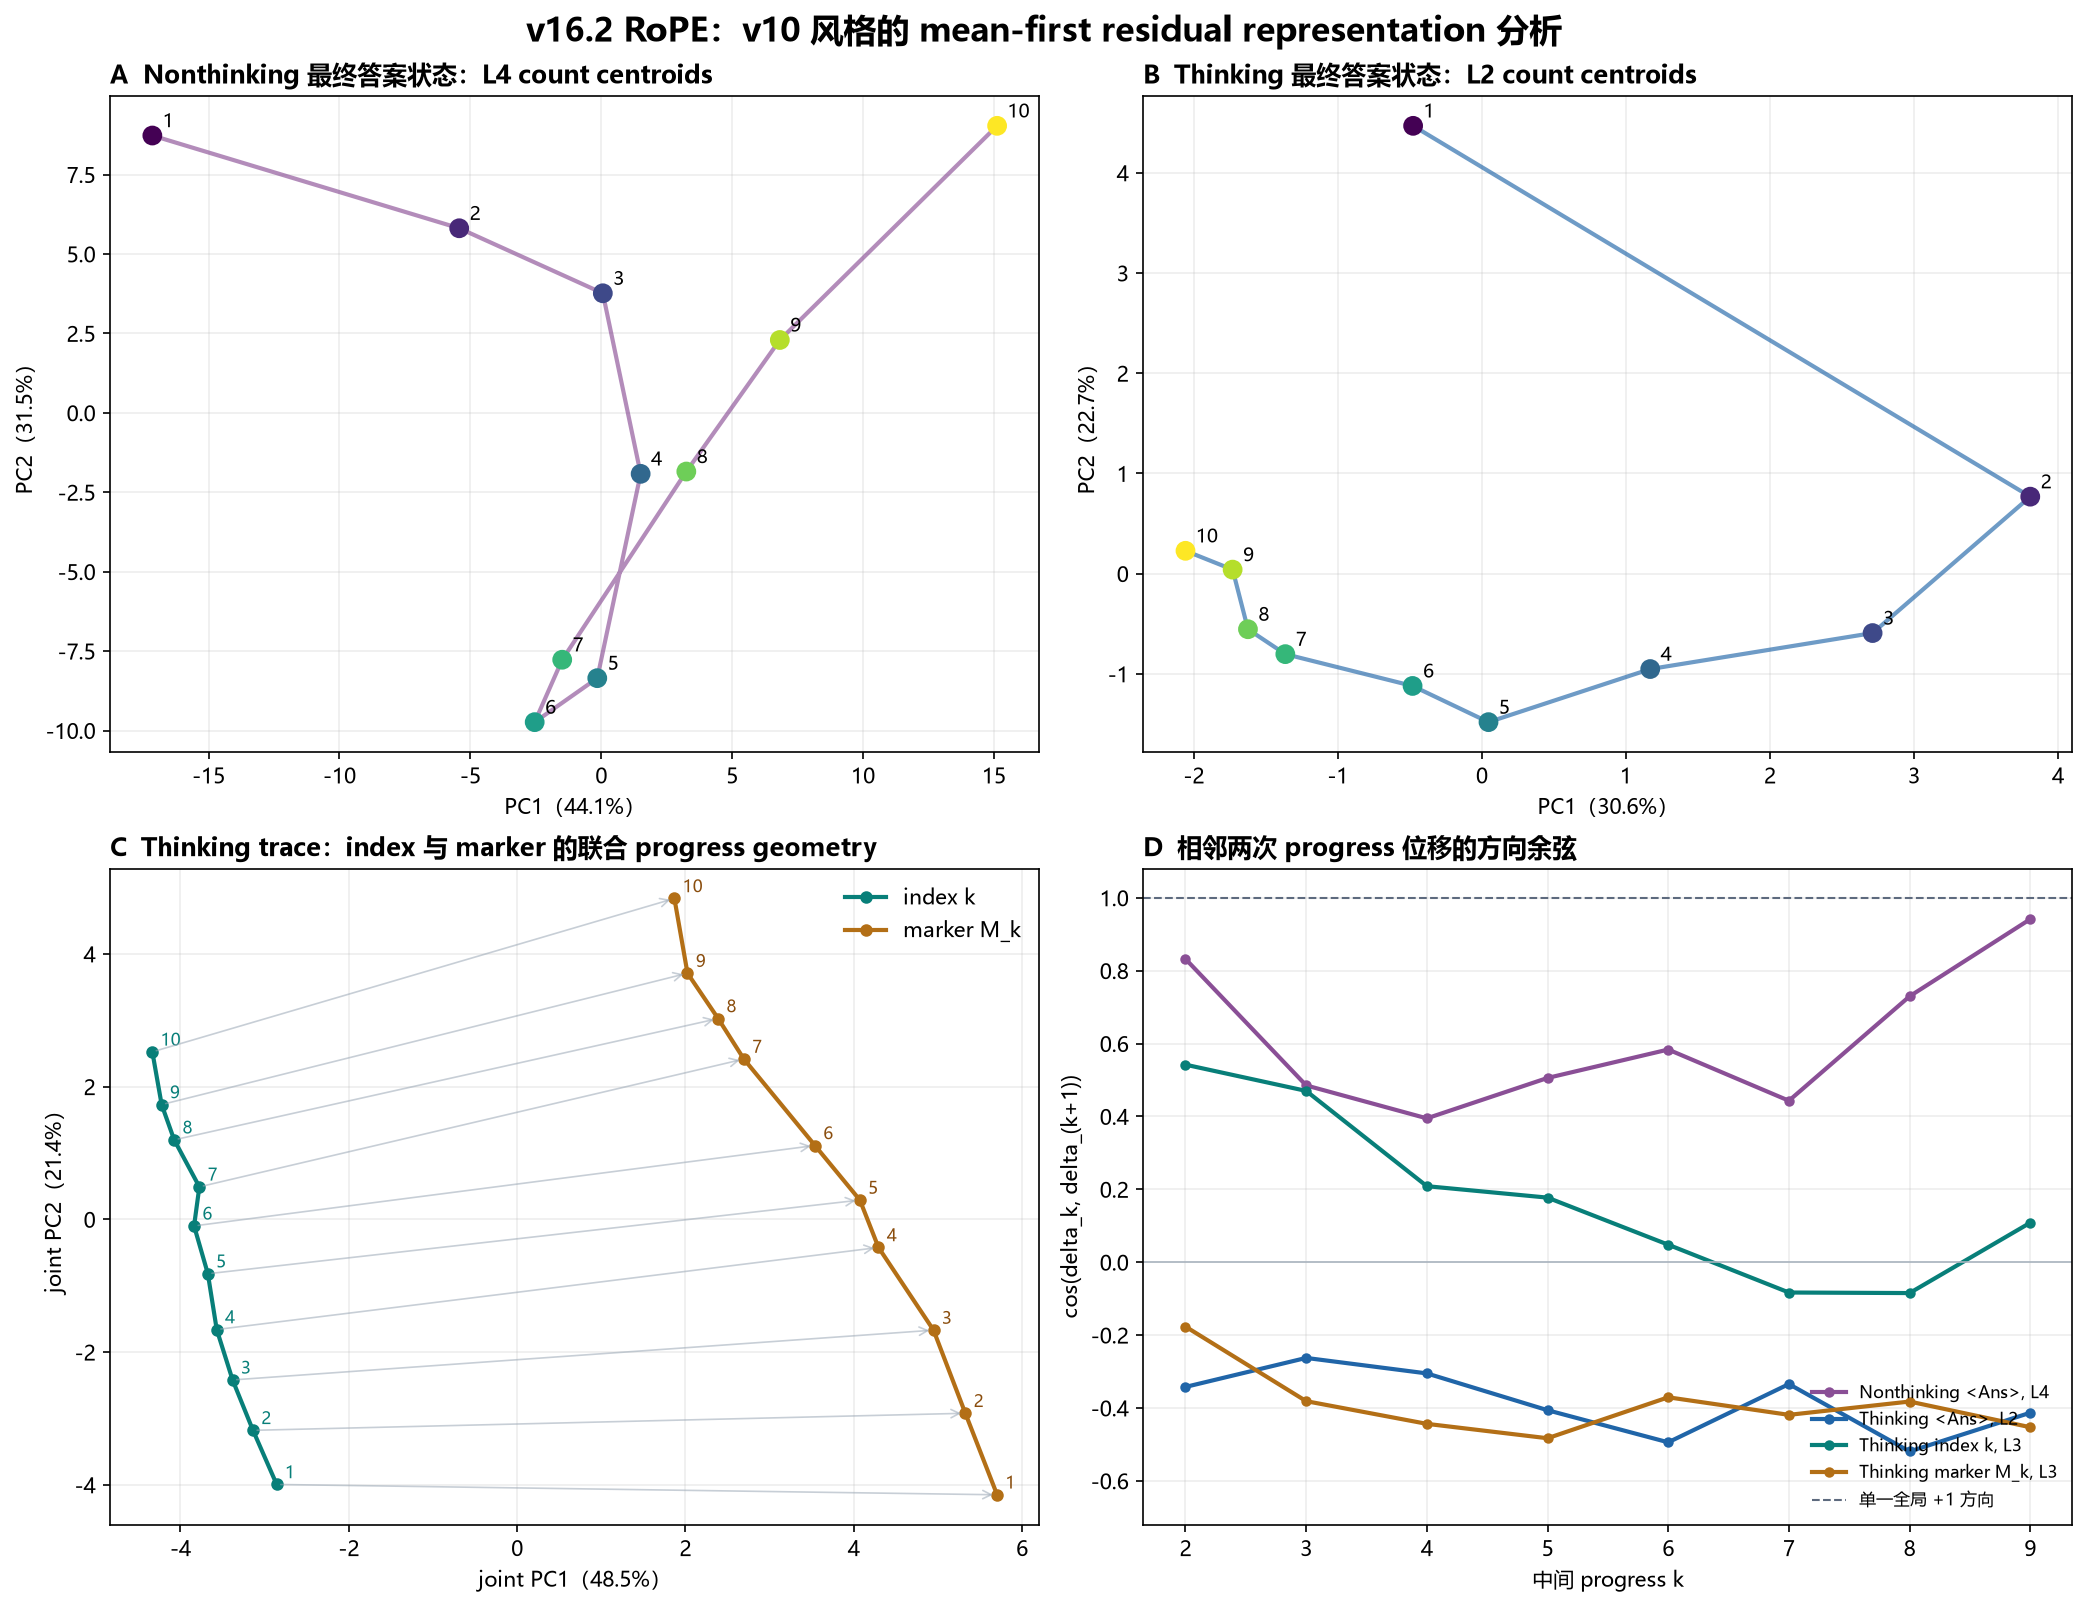
\includegraphics[width=\linewidth]{figures/synthetic_geometry.png}
    \end{minipage}
    \caption{Left: head-to-state damage and state-to-head routing control. Right: mean-first residual geometry across the two representations.}
    \label{fig:app-loop}
\end{figure}

\begin{figure}[h]
    \centering
    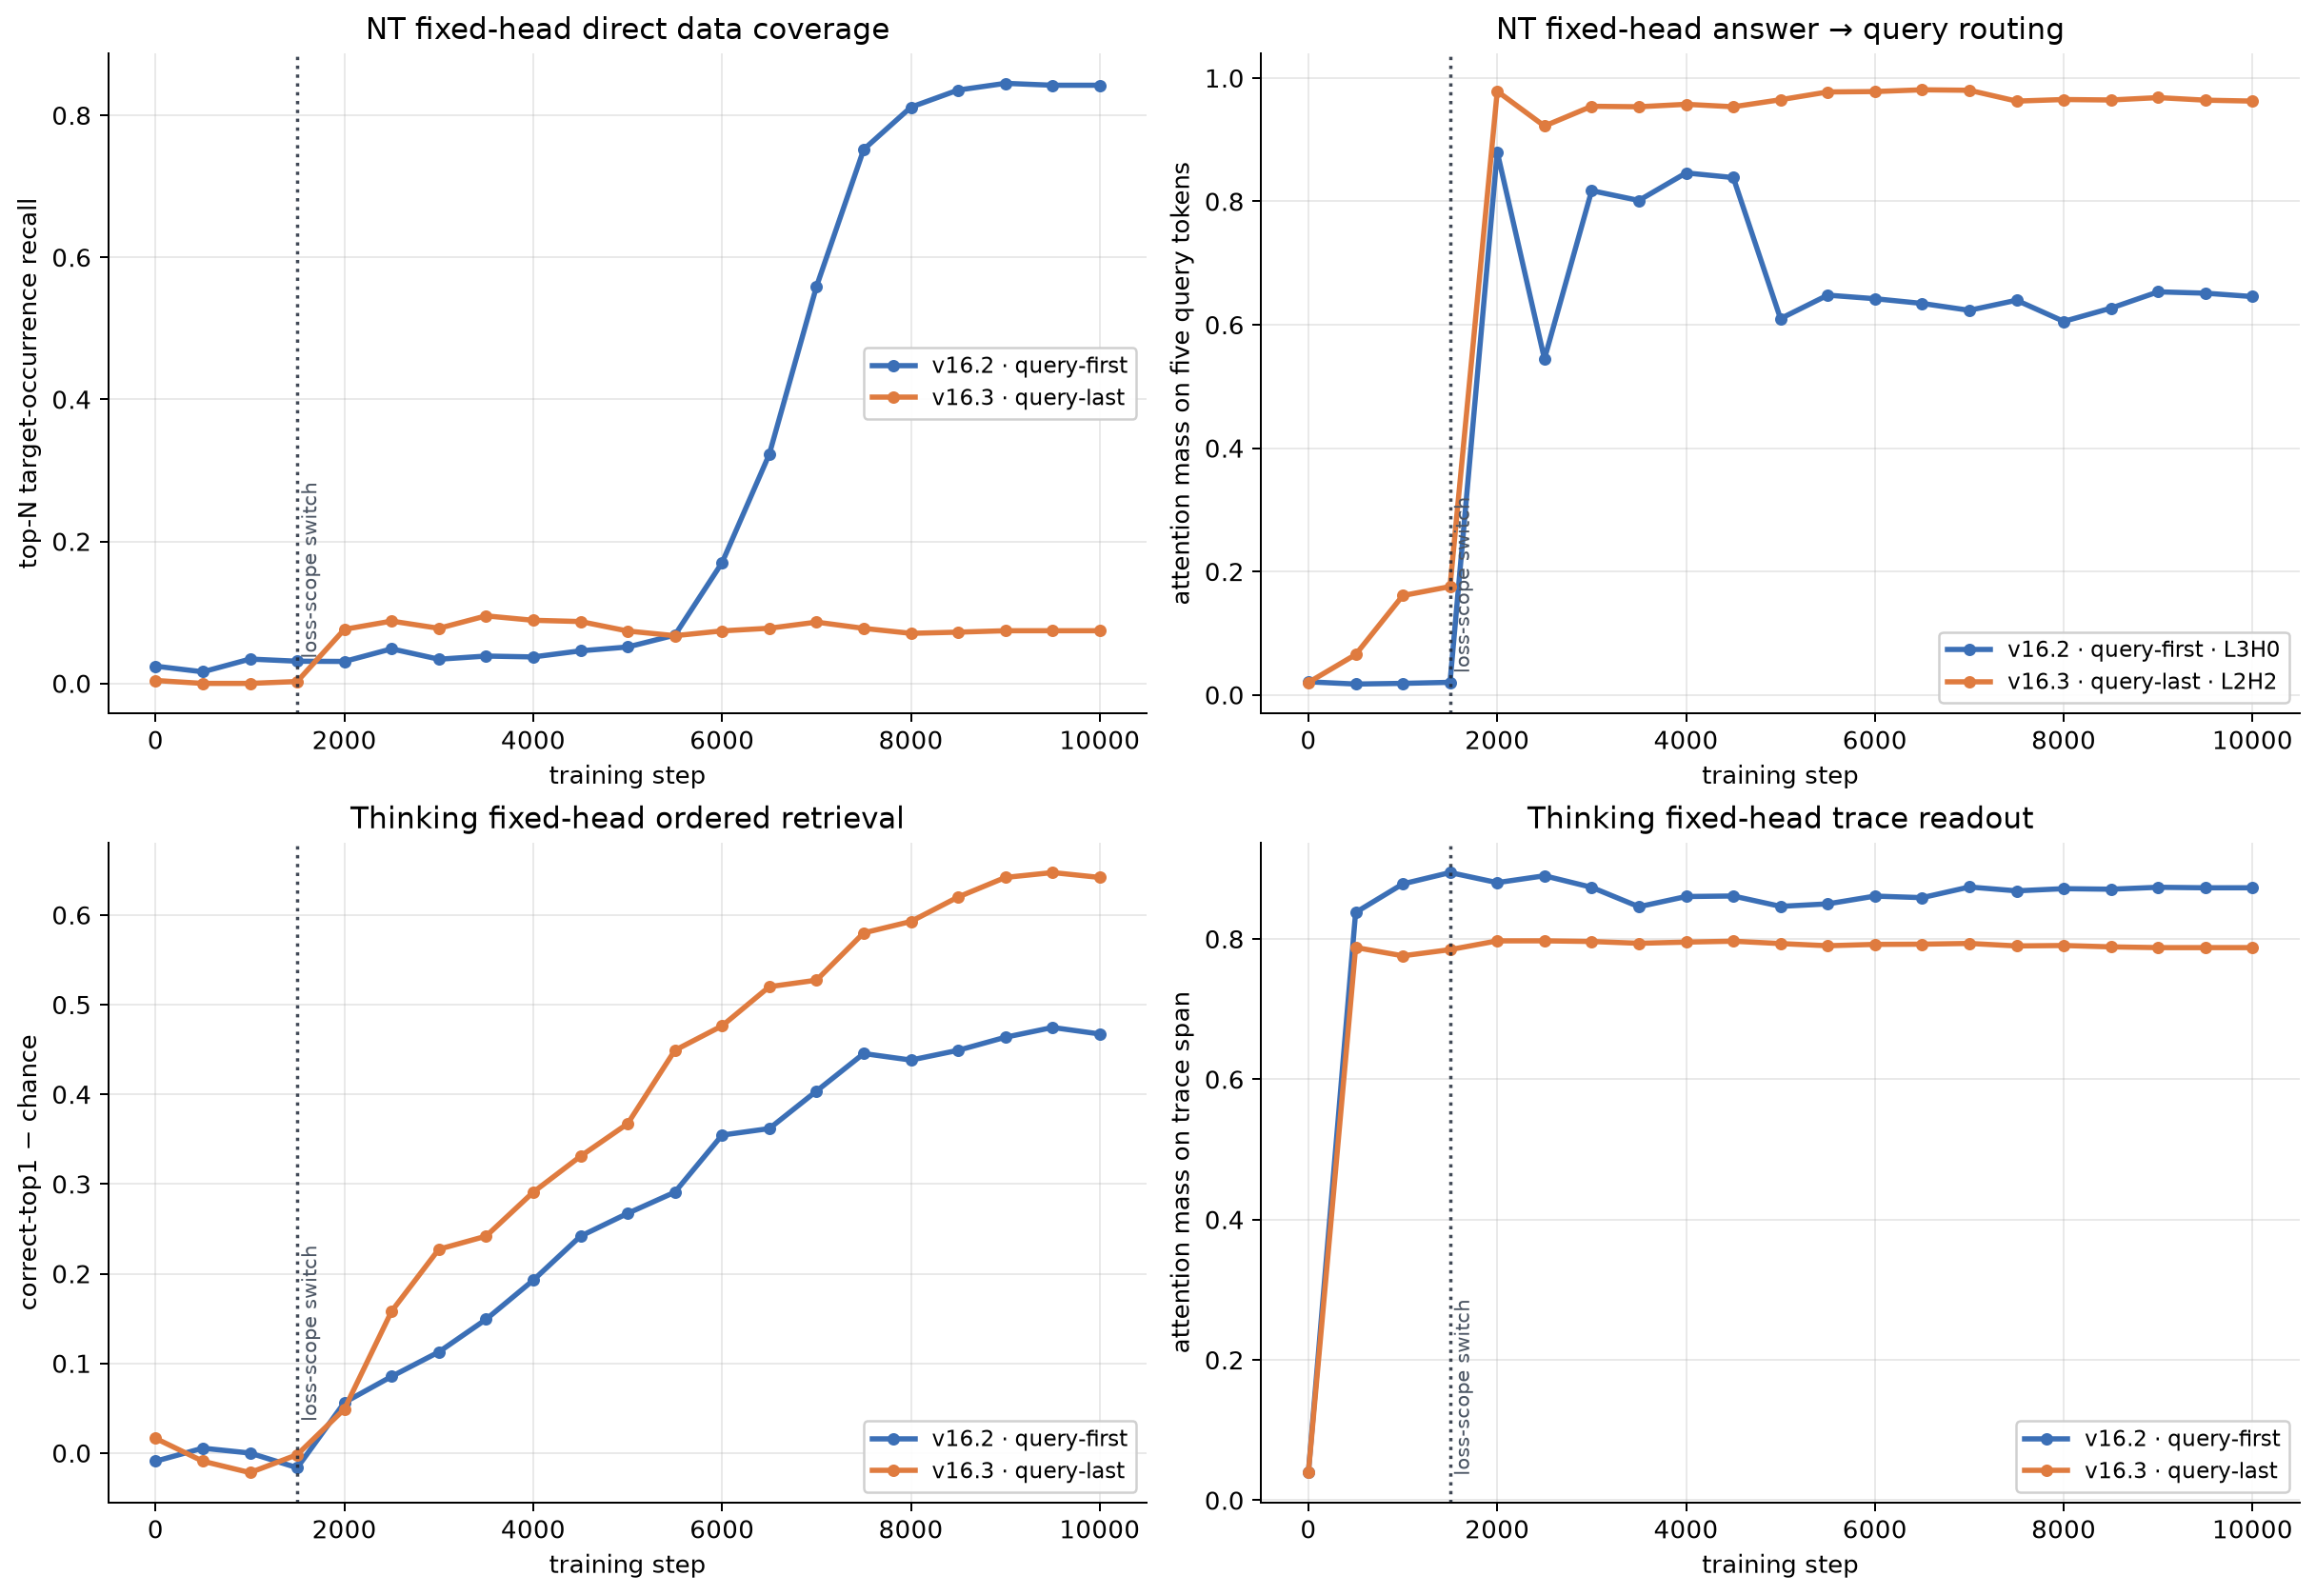
\includegraphics[width=\linewidth]{figures/query_order_routes.png}
    \caption{Fixed-head route dynamics under query-first and query-last layouts. Query-last weakens direct data coverage and strengthens answer-to-query routing while improving thinking ordered retrieval.}
    \label{fig:app-query-route}
\end{figure}

\clearpage
\section{Additional realistic-model results}

\begin{figure}[h]
    \centering
    \begin{minipage}[t]{0.49\linewidth}
        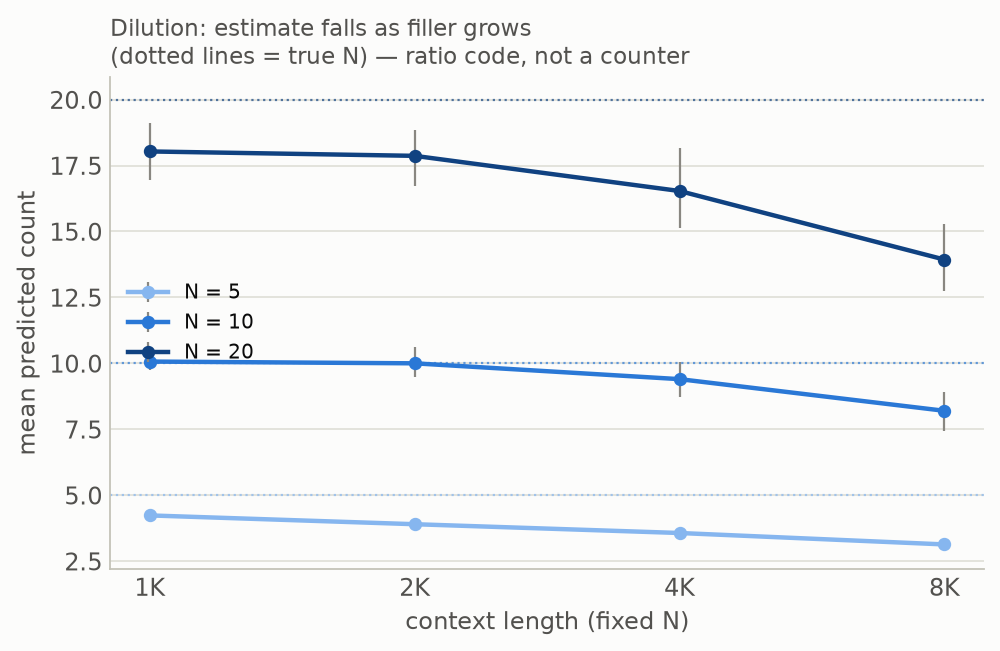
\includegraphics[width=\linewidth]{figures/realistic_dilution.png}
    \end{minipage}\hfill
    \begin{minipage}[t]{0.49\linewidth}
        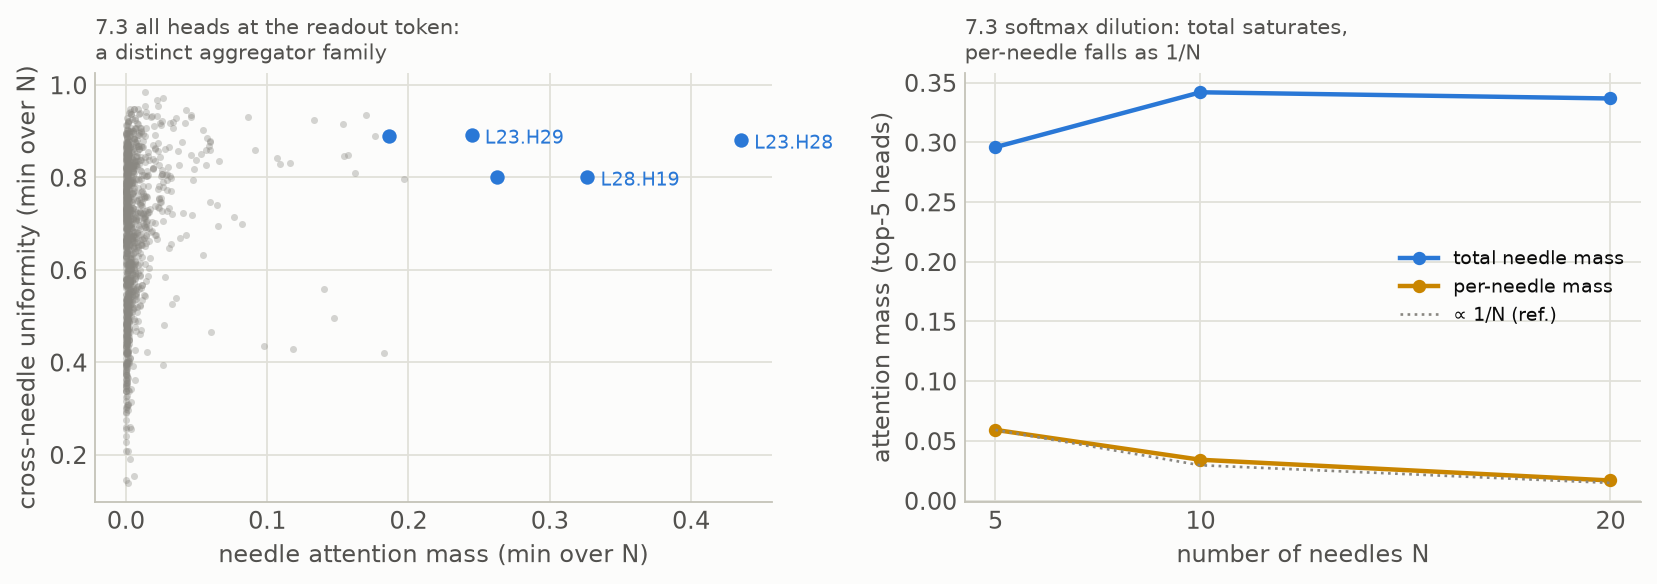
\includegraphics[width=\linewidth]{figures/realistic_attention_aggregators.png}
    \end{minipage}
    \caption{At fixed $N$, additional filler dilutes the predicted count. Readout heads have high cross-needle uniformity; total target mass saturates and per-needle mass follows an approximate $1/N$ law.}
    \label{fig:app-real-direct}
\end{figure}

\begin{figure}[h]
    \centering
    \begin{minipage}[t]{0.49\linewidth}
        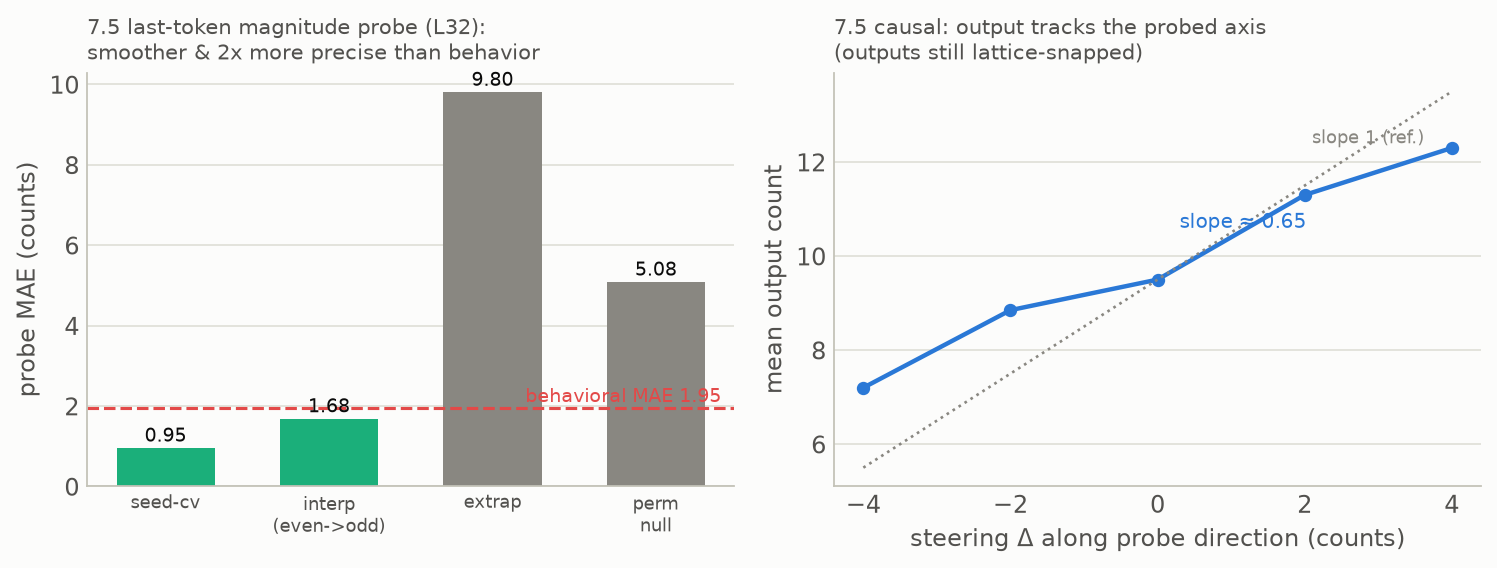
\includegraphics[width=\linewidth]{figures/realistic_steering.png}
    \end{minipage}\hfill
    \begin{minipage}[t]{0.49\linewidth}
        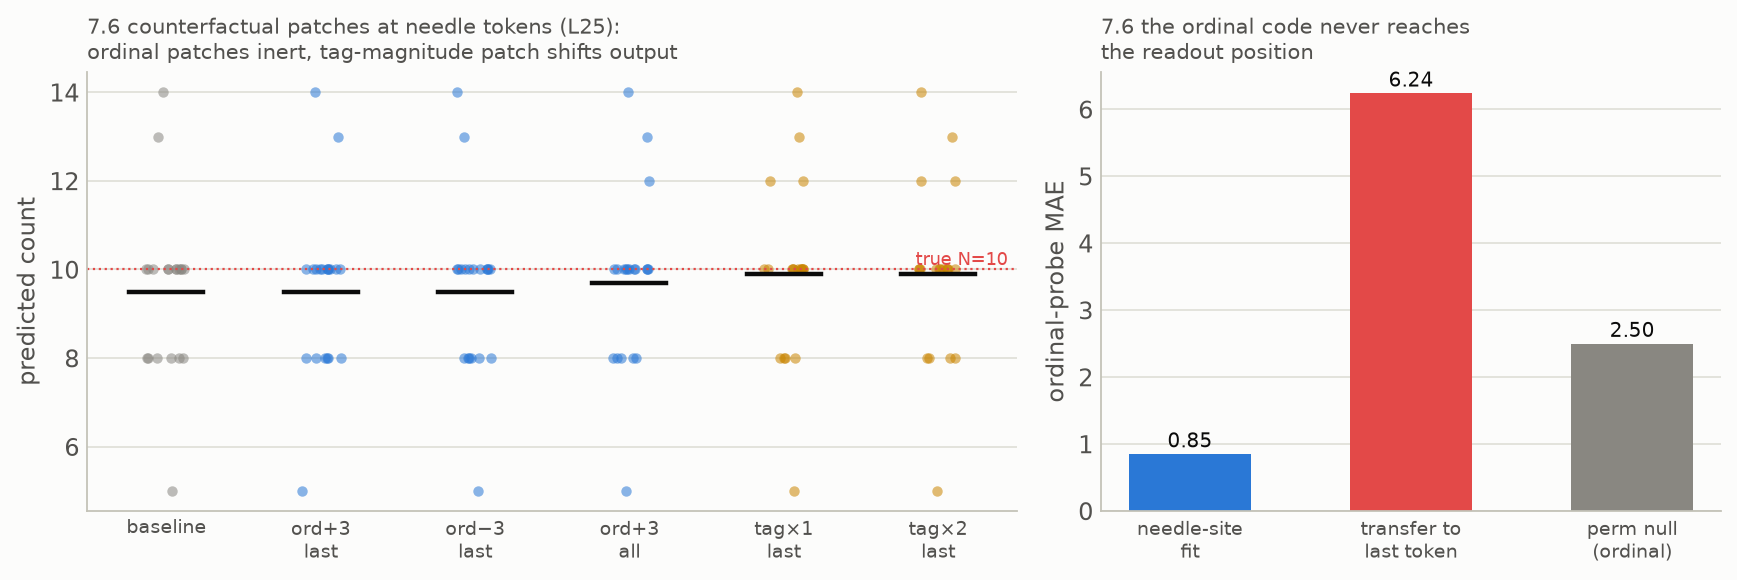
\includegraphics[width=\linewidth]{figures/realistic_ordinal_patch.png}
    \end{minipage}
    \caption{Realistic Qwen interventions. Final-token magnitude steering controls the emitted count, but ordinal directions found at needle sites do not transfer to the readout; tag-strength patches at the same site do affect output.}
    \label{fig:app-real-causal}
\end{figure}

\begin{figure}[h]
    \centering
    \begin{minipage}[t]{0.49\linewidth}
        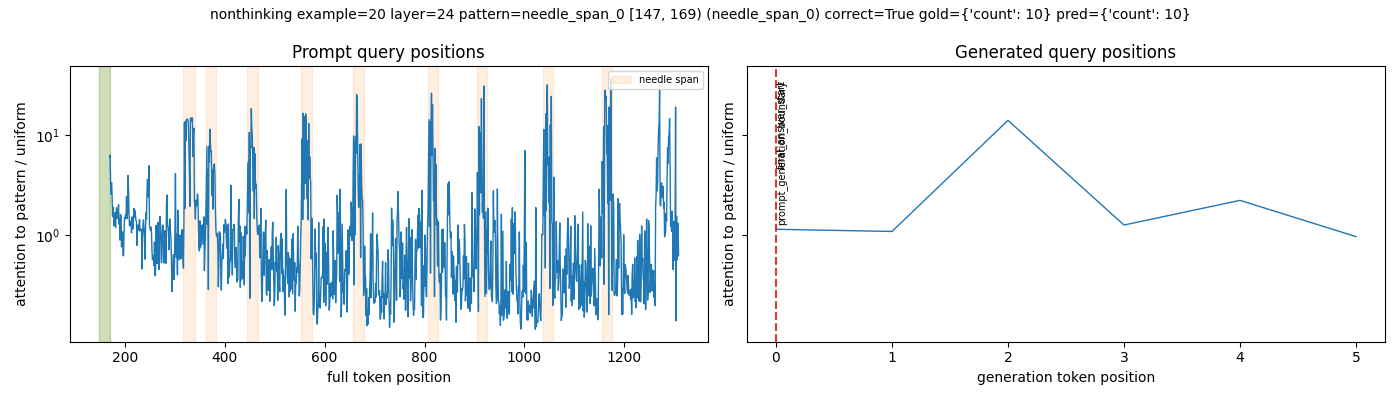
\includegraphics[width=\linewidth]{figures/qwen_broad_attention.png}
    \end{minipage}\hfill
    \begin{minipage}[t]{0.49\linewidth}
        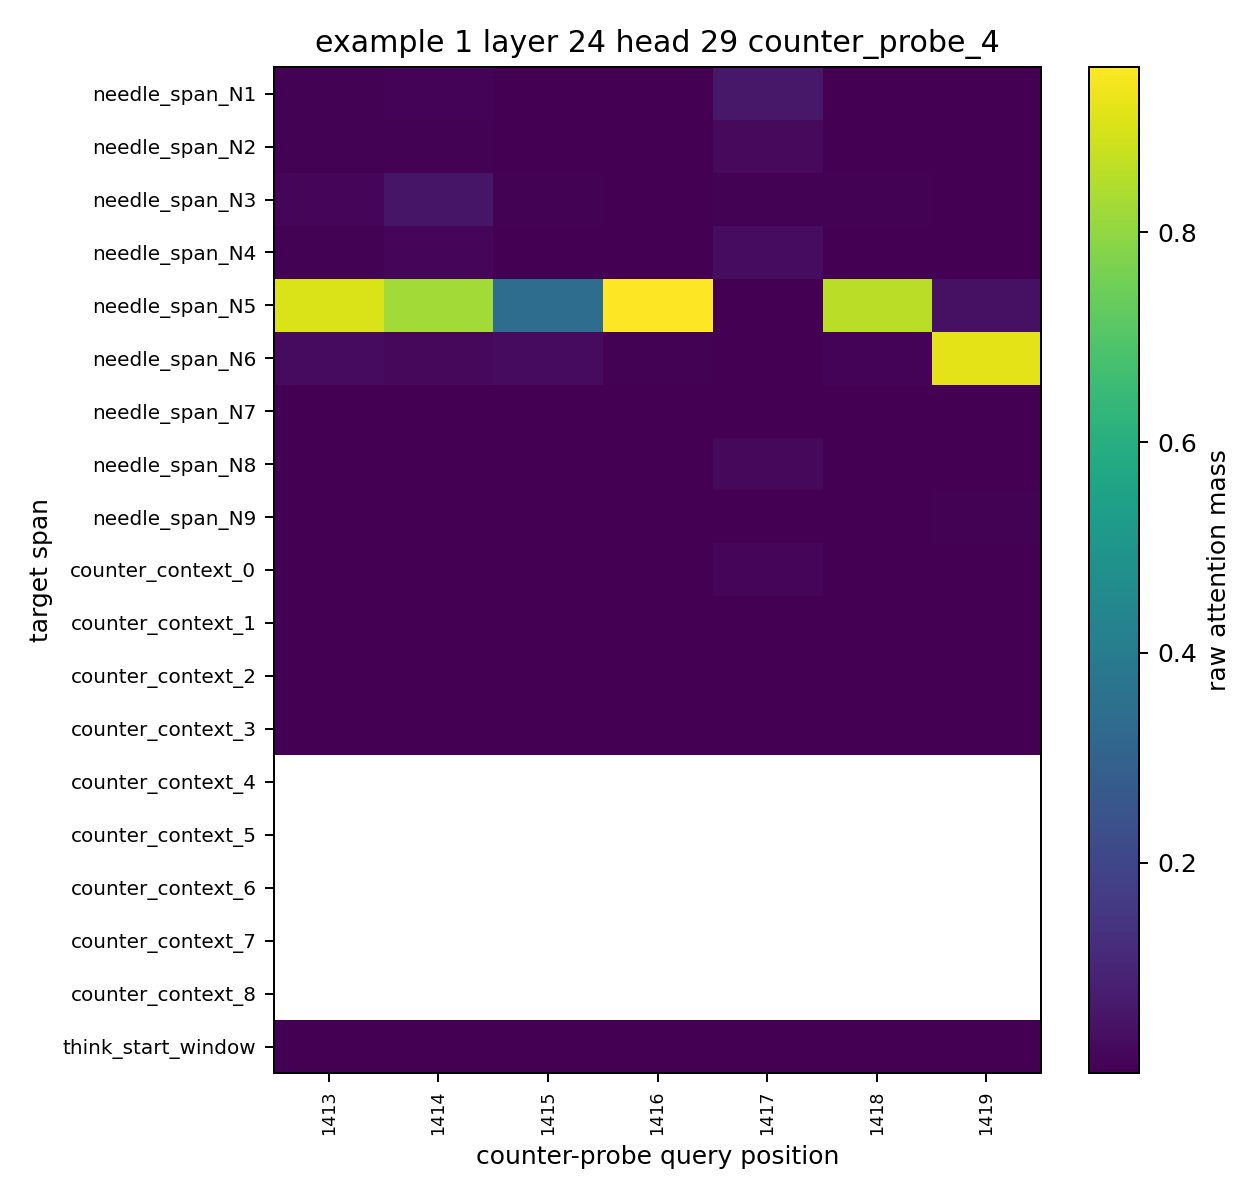
\includegraphics[width=\linewidth]{figures/qwen_targeted_attention.png}
    \end{minipage}
    \caption{Qualitative attention contrast in Qwen3-8B: broad prompt-needle attention without a trace (left) and more targeted prompt retrieval from indexed CoT spans (right). These plots motivate roles but do not replace the controlled causal tests.}
    \label{fig:app-real-attention}
\end{figure}

\clearpage
\section{Claim--evidence matrix and highest-value next experiments}

\begin{table}[H]
\caption{Current evidence strength. ``Supported'' denotes convergent held-out description and at least one targeted intervention, not a cross-seed theorem.}
\centering
\small
\begin{tabular}{p{1.85in}p{1.0in}p{2.25in}}
\toprule
Claim & Status & Principal remaining test \\
\midrule
Direct answers use broad set routing & Supported & Replicate role/subspace across $\geq5$ seeds \\
Trace indices support ordered retrieval & Supported & Patch natural AR errors and decompose Q/K/V \\
Progress state controls later retrieval & Partial causal & Path-specific mediation with alternate routes blocked \\
Trace span determines final scalar count & Supported but confounded & Fix answer position while varying valid pair count \\
Query-last creates a query bottleneck & Convergent indirect & Probe and patch query-token states directly \\
Realistic bare count uses parallel ratio code & Supported in Qwen & Cross-model causal replication and 16K/32K tests \\
CoT mechanism transfers unchanged to LLMs & Suggestive & Full ablation/patch/steer battery in multiple LLMs \\
\bottomrule
\end{tabular}
\end{table}

Highest-value experiments are: (1) repeat the controlled role ranking, top-2 readout synergy, and L2/L4 transport onset for at least five seeds using permutation-invariant head-subspace comparisons; (2) train with padding or masks that vary valid trace-pair count while keeping \ans{} and RoPE distances fixed; (3) collect and intervene on query-token states in the query-last layout; (4) repeat interventions on naturally occurring held-out AR errors; and (5) extend the realistic causal battery to additional model families and longer contexts.

\end{document}
